\documentclass[10pt,twoside]{book}
\usepackage[utf8]{inputenc}
\usepackage[latin,spanish]{babel}
\usepackage[T1]{fontenc}
\usepackage{fontspec}
\usepackage{blindtext}
\usepackage{hyperref}
\hypersetup{
    hidelinks,
    pdftitle={Santo Rosario y \'Angelus},
    pdfauthor={Sergio},
    pdfkeywords={Cat\'olico, Santa Mar\'ia, Santo Rosario},
    pdfcreator={VS Code + LuaTeX}
}
\usepackage[spanish]{cleveref}
\usepackage{geometry}
\usepackage{setspace}
\geometry{
    a4paper,
    inner=15mm,
    outer=10mm,
    top=15mm,
    bottom=15mm
}
\usepackage{paracol}
\usepackage{lettrine}
\usepackage{xcolor}
\usepackage{gregoriotex}
\usepackage{graphicx}
\graphicspath{ {images/} }
\usepackage{fancyhdr}
\pagestyle{fancy}
\fancyhf{}
\fancyfoot[LE,RO]{\thepage}
\renewcommand{\headrulewidth}{0pt}
\renewcommand{\footrulewidth}{0pt}

\setlength{\columnseprule}{0.4pt}
\colseprulecolor{red}


\usepackage{datetime}
\newdateformat{monthyeardate}{%
  \monthname[\THEMONTH] \THEYEAR
}
\newcommand{\primeraletragranderoja}[2]{
    \lettrine[lines=2]{\textcolor{red}{#1}}{#2}
}

\newcommand{\primeraletragranderojasola}[1]{
    \lettrine[lines=2]{\textcolor{red}{#1}}{}
}

\newcommand{\primeraletragrande}[2]{
    \lettrine[lines=2]{#1}#2
}

\newcommand{\letraroja}[2]{
    \textcolor{red}{#1}#2
}

\newcommand{\versiculo}[1]{
    \textcolor{red}{\Vbar.} #1.
}

\newcommand{\respuesta}[1]{
    \textcolor{red}{\Rbar.} #1.
}

\newcommand{\textopequenorojo}[1]{
    {\textcolor{red}{\small{#1}}}
}

\newcommand{\versiculorespuesta}[2]{
    \versiculo{#1}\\
    \respuesta{#2}
}

\newcommand{\versiculorespuestaseguido}[2]{
    \versiculo{#1}\respuesta{#2}
}

\newcommand{\redcross}{
    \textcolor{red}{\grecross}
}

\newcommand{\lineahorizontal}[2]{
    \begin{center}
        {\rule{#1cm}{#2pt}}
    \end{center}
}

\newcommand{\lineahorizontalroja}[2]{
    \begin{center}
        \textcolor{red}{\rule{#1cm}{#2pt}}
    \end{center}
}

\newcommand{\latinderecha}[1]{
    \begin{otherlanguage}{latin}
        \begin{rightcolumn}
            \input{#1}    
        \end{rightcolumn}
    \end{otherlanguage}
}

\newcommand{\castellanoizquierda}[1]{
    \begin{leftcolumn}
        \input{#1}
    \end{leftcolumn}
}

\newcommand{\castellanoizquierdasincro}[1]{
    \begin{leftcolumn*}
        \input{#1}
    \end{leftcolumn*}
}

\newcommand{\castellanoizquierdasincronota}[2]{
    \begin{leftcolumn*}[#1]
        \input{#2}
    \end{leftcolumn*}
}

\newcommand{\filacastellanolatin}[2]{
    {    
        \begin{leftcolumn}
            \input{#1}
        \end{leftcolumn}
        \begin{otherlanguage}{latin}
            \begin{rightcolumn}
                \input{#2}    
            \end{rightcolumn}
        \end{otherlanguage}
    }
}

\newcommand{\filacastellanolatinsincro}[2]{
    {    
        \begin{leftcolumn*}
            \input{#1}
        \end{leftcolumn*}
        \begin{otherlanguage}{latin}
            \begin{rightcolumn}
                \input{#2}    
            \end{rightcolumn}
        \end{otherlanguage}
    }
}

\newcommand{\filacastellanolatinsincronota}[3]{
    \castellanoizquierdasincronota{#1}{#2}
    \latinderecha{#3}
}

\newcommand{\titulomisterios}[2]{
    {    
        \begin{minipage}[t]{0.595\textwidth}
            \subsection*{#1}
        \end{minipage}\begin{minipage}[t]{0.395\textwidth}
            \begin{flushright}
                \textcolor{red}{#2}
            \end{flushright}
        \end{minipage}
    }
}

\newcommand{\titulomisterio}[2]{
    {
        \begin{minipage}[t]{0.595\textwidth}
            \section*{#1}
        \end{minipage}\begin{minipage}[t]{0.395\textwidth}
            \begin{flushright}
                \textcolor{red}{#2}
            \end{flushright}
        \end{minipage}
    }
}

\newcommand{\iralfinal}{
    \begin{center}
        \textcolor{red}{Una vez terminamos nos vamos a la \cpageref{final-prayer} para las oraciones finales.}
    \end{center}
}





\begin{document}

\begin{titlepage}
      \begin{center}

            \vspace*{10em}

            {\Huge \uppercase{Santo Rosario y Ángelus}}

            \vspace{1.5em}

            {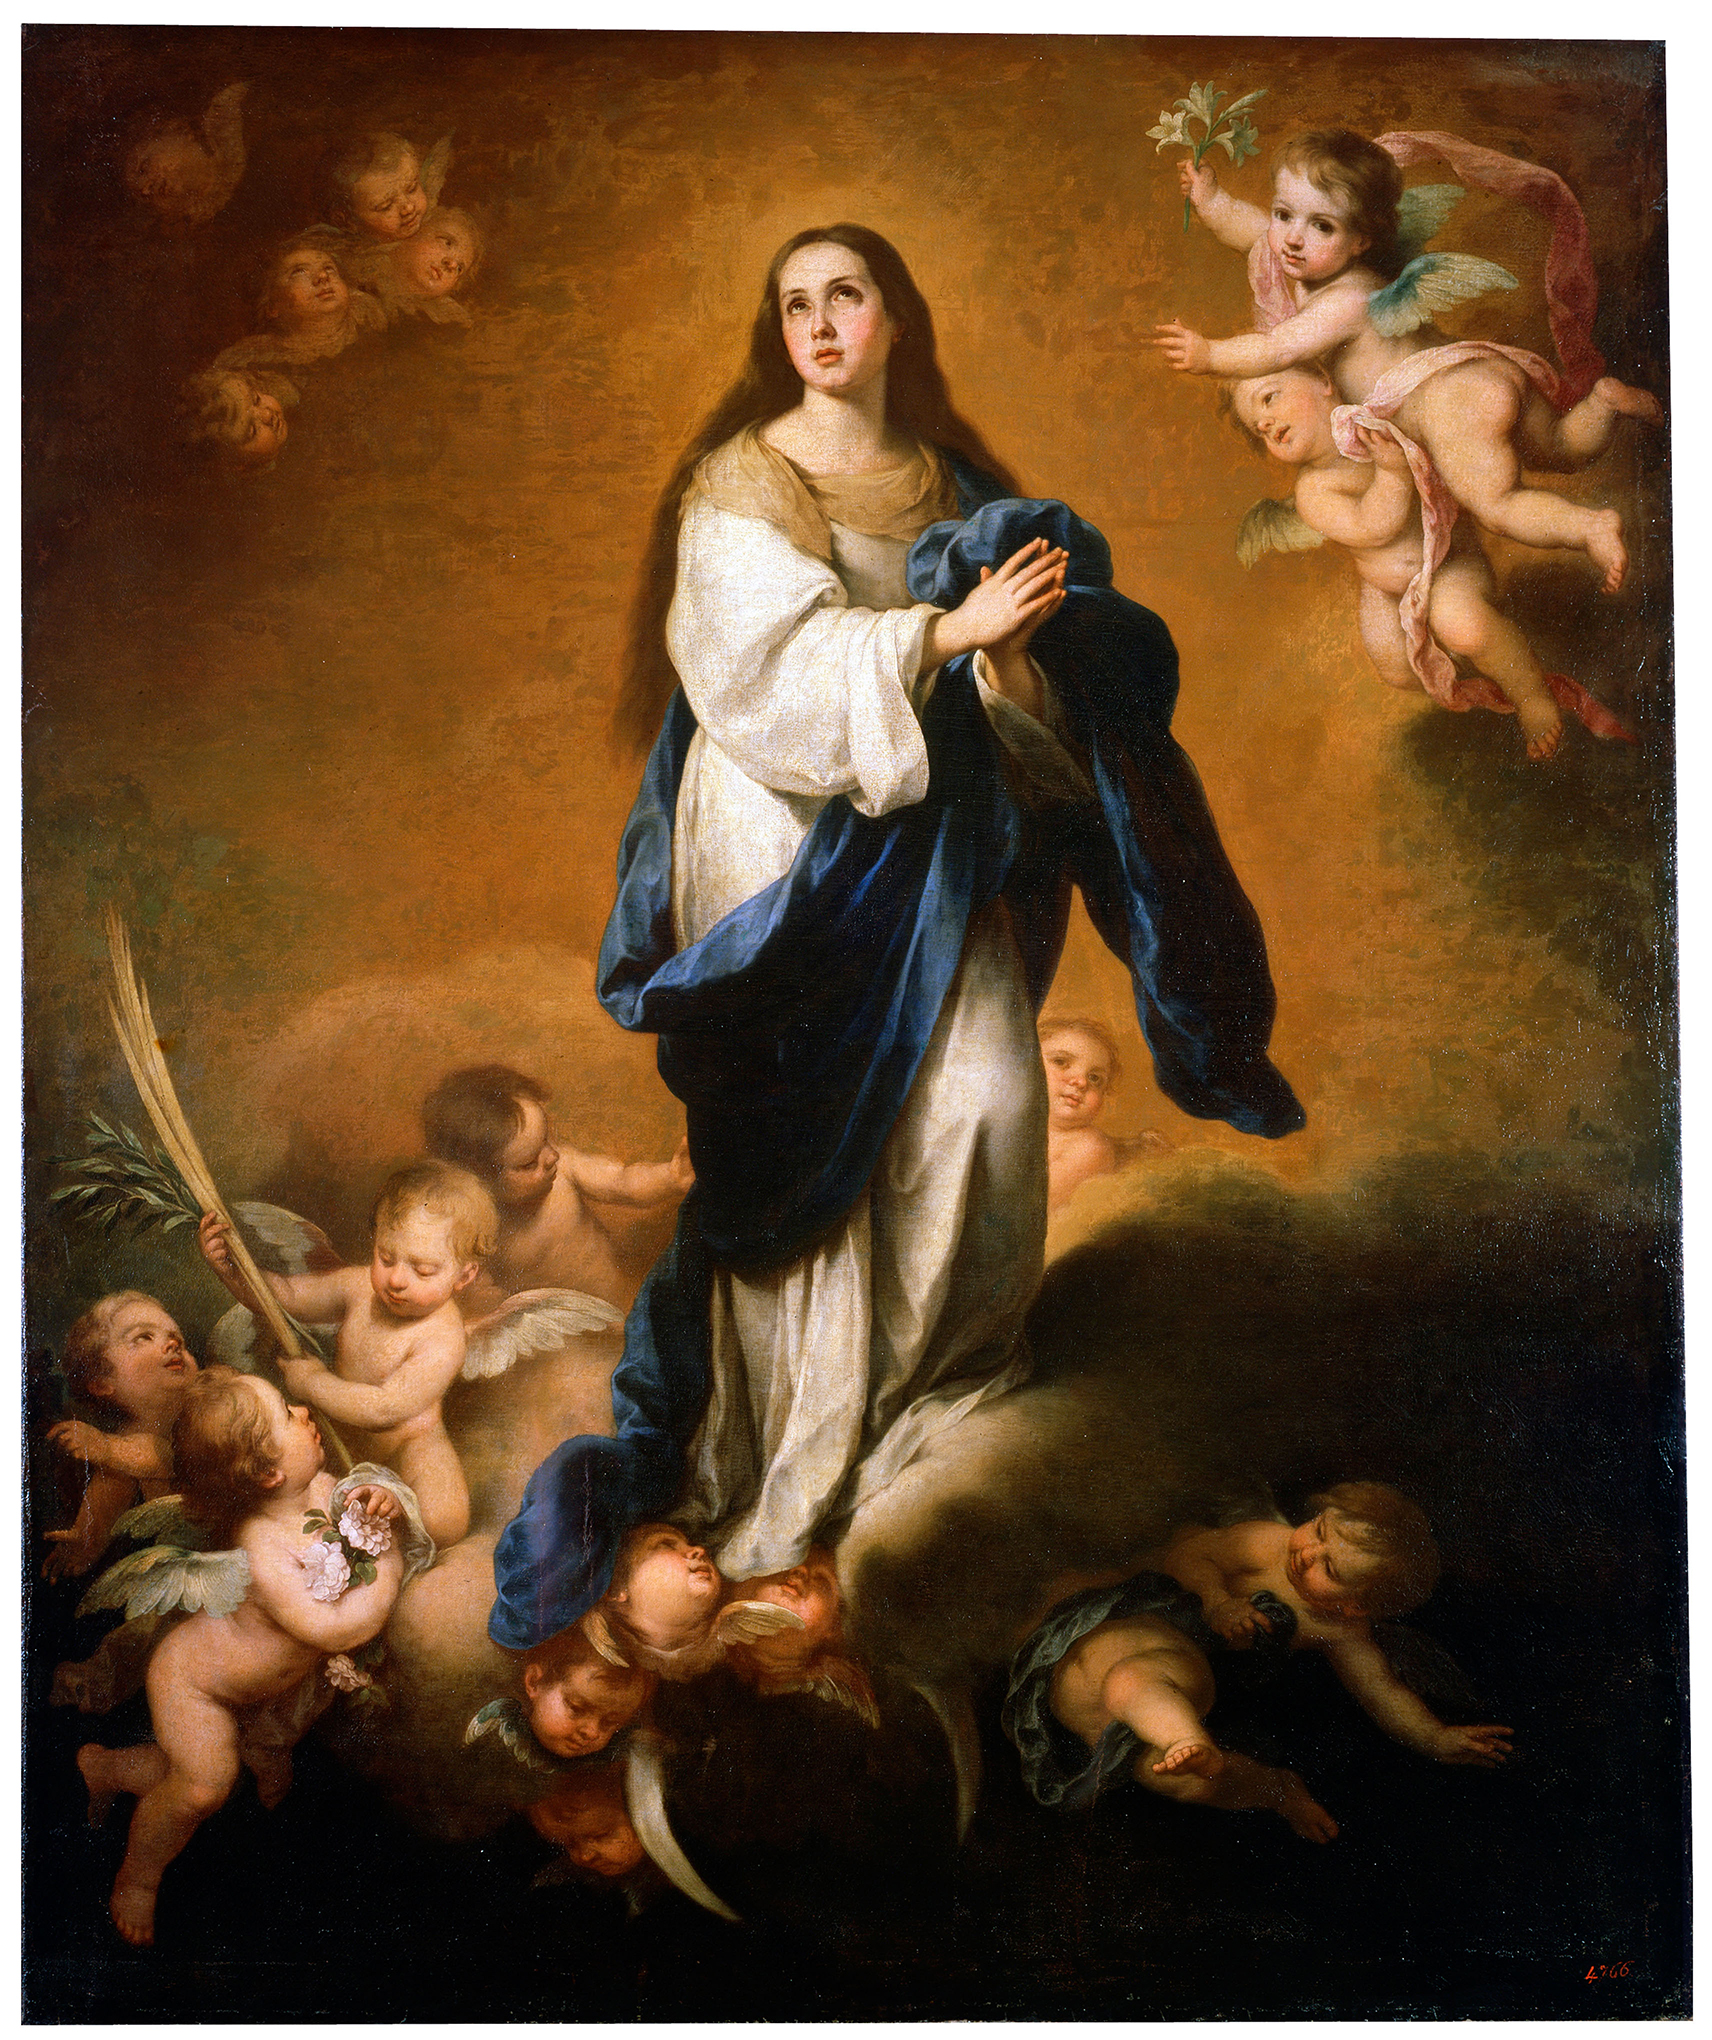
\includegraphics[scale=0.95]{foto-04.jpg}}

            \vspace{0.5em}

            Sergio

            Valladolid (España), \monthyeardate\today
      \end{center}
\end{titlepage}
\twosided{c}
\footnotelayout{m}

\chapter*{\centering\textcolor{red}{S}anto \textcolor{red}{R}osario \textcolor{red}{M}editado}

\begin{paracol}{2}

      \ensurevspace{20mm}

      \begin{leftcolumn}
            En el Nombre del Padre, y del{\redcross}Hijo, y del Espíritu Santo. Amén.
      \end{leftcolumn}
      \begin{otherlanguage}{latin}
            \begin{rightcolumn}
                  In Nómine Pátris, et{\redcross}Filii, et Spíritus Sancti. Amen    
            \end{rightcolumn}
      \end{otherlanguage}

      \definecolumnpreamble{0}{\vspace{0.5em}}
      \definecolumnpreamble{1}{\vspace{0.5em}}

      \begin{leftcolumn*}
            \primeraletragranderoja{S}{eñor}mío Jesucristo, Dios y Hombre verdadero, Creador y Redentor mío: por ser vos quién sois, y porque os amo sobre todas las cosas,
me pesa de todo corazón de haberos ofendido, propongo firmemente nunca más pecar, y apartarme de todas las ocasiones de ofenderos,
confesarme, y cumplir la penitencia que me fuere impuesta; ofrézcoos mi vida, obras y trabajos en satisfacción de todos mis pecados;
y confío en vuestra bondad y misericordia infinita me los perdonaréis por los merecimientos de vuestra preciosísima sangre, pasión y muerte,
y me daréis gracia para enmendarme y para perseverar en vuestro santo servicio hasta el fin de mi vida. Amén.\footnote{\label{contricion}En vez del \textit{Señor mio, Jesucristo} o del \textit{Confíteor}, podemos rezar:\\ \indent\textcolor{red}{D}ios mío, me arrepiento de todo corazón de todos mis pecados y los aborrezco, porque al pecar, no sólo merezco las penas establecidas 
por ti justamente, sino principalmente porque te ofendí, a ti sumo Bien y digno de amor por encima de todas las cosas. Por eso propongo firmemente, 
con ayuda de tu gracia, no pecar más en adelante y huir de toda ocasión de pecado. Amén.\\ \indent En latín:\\ \indent\textcolor{red}{D}eus meus, ex toto corde p{\ae}nitet me ómnium meórum peccatórum, éaque detéstor, quia peccándo, non solum pœnas a te iuste statútas 
proméritus sum, sed pr{\ae}sértim quia offéndi te, summum bonum, ac dignum qui super ómnia diligáris. Ídeo fírmiter propóno, adiuvánte grátia tua, 
de cétero me non peccatúrum peccandíque occasiónes próximas fugitúrum. Amen.}
      \end{leftcolumn*}
      \begin{otherlanguage}{latin}
            \begin{rightcolumn}
                \primeraletragranderoja{C}{onfíteor}Deo omnipoténti, beát{\ae} Marí{\ae} semper Virigini, beáto Michaéli Archángelo, beáto Joánni Baptíst{\ae}, sanctis 
Apóstolis Petro et Paulo, ómníbus Sanctis, quia peccávi nimis, cogitatióne, verbo et ópere, mea culpa, mea culpa, mea máxima culpa. Ideo precor beátam
Maríam semper Virgínem, beátum Michaélem Archángelum, beátum Joánnem Baptístam, sanctis Apóstolos Petrum et Paulum, omnes Sanctos,
oráre pro me ad Dóminum Deum nostrum.\\
Misereátur nostri omnipotens Deus, et, dimíssis peccátis nostris, perdúcat nos ad vitam {\ae}térnam. Amen.\\
Indulgéntiam, absolutionem, et remissiónem peccatórum nostrórum tríbuat nobis omnípotens et miséricors Dóminus. Amen.(\cref{contricion})
            \end{rightcolumn}
      \end{otherlanguage}

      \begin{leftcolumn*}
            \versiculorespuestaseguido{Abre, Señor, mis labios}{Y mi boca cantará tus alabanzas}
      \end{leftcolumn*}
      \begin{otherlanguage}{latin}
            \begin{rightcolumn}
                \versiculorespuestaseguido{Dómine, lábia mea apéries}{Et os meum annuntiábit laudem tuam}
            \end{rightcolumn}
      \end{otherlanguage}

      \begin{leftcolumn*}
            \versiculorespuestaseguido{Apresútare, Señor, a socorrerme}{Ven, oh Dios, en mi ayuda}
      \end{leftcolumn*}
      \begin{otherlanguage}{latin}
            \begin{rightcolumn}
                \versiculorespuestaseguido{Deum, in adjutórium meum inténde}{Dómine, ad adjuvándum me festina}
            \end{rightcolumn}
      \end{otherlanguage}

      \begin{leftcolumn*}
            \versiculorespuestaseguido{Gloria al Padre, al Hijo, y al Espíritu Santo}{Como era en el principio, ahora, y siempre, y por los siglos de los siglos. Amén}
      \end{leftcolumn*}
      \begin{otherlanguage}{latin}
            \begin{rightcolumn}
                \versiculorespuestaseguido{Glória Patri, et Filio, et Spirítui Sancto}{Sicut erat in princípio et nunc, et semper et in s{\ae}cula s{\ae}culórum. Amen}
            \end{rightcolumn}
      \end{otherlanguage}

      \begin{leftcolumn*}
            \versiculorespuestaseguido{María, Madre de gracia, Madre de Misericordia}{Defendednos del enemigo y amparadnos ahora y en la hora de nuestra muerte. Amén}
      \end{leftcolumn*}
      \begin{otherlanguage}{latin}
            \begin{rightcolumn}
                \versiculorespuesta{María Mater grati{\ae}, Mater Misericordi{\ae}}{Tu nos ab hoste protege et mortis hora súspice. Amen}
            \end{rightcolumn}
      \end{otherlanguage}
      \definecolumnpreamble{0}{\vspace{0em}}
      \definecolumnpreamble{1}{\vspace{0em}}
\end{paracol}

\vspace{0.5em}

\begin{center}
      \textcolor{red}{Decimos aquí las intenciones de este Rosario}
\end{center}

\section*{\centering Dominica (Domingo)}

\noindent\subsection*{Misterio Gloriosos}

\noindent\subsubsection*{I La Resurrección del Señor}

\vspace{-0.5em}

\hfill\textcolor{red}{Mt 28, 1-3.5-7}

\lettrine[lines=2]{\textcolor{red}{P}}asado el sábado, ya para amanecer el día primero de la semana, vino María Magdalena con la otra María al sepulcro. Y sobrevino un gran terremoto,
pues un ángel del Señor bajó del cielo y acercándose removió la piedra del sepulcro y se sentó sobre ella. Era su aspecto como el relámpago, y su vestidura blanca como la nueve.
El ángel, dirigiéndose a las mujeres, dijo: No temáis vosotras, pues sé que buscáis a Jesús el crucificado. No está aquí; ha resucitado, según lo había dicho.
Venid y ved el sitio donde fue puesto. Id luego y decid a sus discípulos que ha resucitado de entre los muertos y que os precede a Galilea; allí le veréis.
Es lo que tenía que deciros.

\vspace{0.5em}

\begin{paracol}{2}
    \filacastellanolatin{oraciones/padrenuestro/castellano_sencillo.tex}{oraciones/padrenuestro/latin_sencillo.tex}
    \vspace{2mm}
    \filacastellanolatinsincronota{\textcolor{red}{El avemaría se repite 10 veces}}{oraciones/avemaria/castellano_sencillo.tex}{oraciones/avemaria/latin_sencillo.tex}
    \vspace{6mm}
    \filacastellanolatinsincro{oraciones/gloria/castellano_separado.tex}{oraciones/gloria/latin_separado.tex}
    \vspace{2mm}
    \filacastellanolatinsincro{oraciones/versiculos/maria_madre/castellano.tex}{oraciones/versiculos/maria_madre/latin.tex}
\end{paracol}

\vspace{1.5em}

\noindent\subsubsection*{II Las Ascensión Jesucristo a los cielos}

\vspace{-0.5em}

\hfill\textcolor{red}{Lc 24, 50; Mc 16, 15-16.19-20}

\lettrine[lines=2]{\textcolor{red}{L}}os llevó hasta cerca de Betania, y levantando sus manos les bendijo. Y les dijo: Id al mundo entero y predicad el Evangelio a toda la creación.
El que creyere y fuere bautizado, se salvará, mas el que no creyere, será condenado. Con esto el Señor Jesús, después de hablarles, fue elevado al cielo y se sentó a la diestra de Dios.
Y ellos, partiéndose de allí, predicaron por todas partes, cooperando el Señor y confirmando la palabra con las señales que la acompañaban.

\vspace{0.5em}

\begin{center}
    Paternóster, diez Avemarías, Gloria

\end{center}

\begin{paracol}{2}
    \filacastellanolatin{oraciones/maria_madre/castellano_seguido.tex}{oraciones/maria_madre/latin_seguido.tex}
\end{paracol}

\vspace{1.5em}

\noindent\subsubsection*{III La Venida del Espíritu Santo sobre los Apóstoles}

\vspace{-0.5em}

\hfill\textcolor{red}{Jn 14, 26; Hch. 2, 1-4}

\lettrine[lines=2]{\textcolor{red}{M}}as el Paráclito, el Espíritu Santo, que enviará el Padre en mi nombre, Él os enseñará todas las cosas y os recordará todas las cosas que os dije yo.
Y al cumplirse el día de Pentecostés, estaban todos juntos en el mismo lugar. Y se produjo de súbito desde el cielo un estruendo como de viento que soplaba vehementemente,
y llenó toda la casa donde se hallaban sentados. Y vieron aparecer lenguas como de fuego, que, repartiéndose, se posaban sobre cada uno de ellos.

\vspace{0.5em}

\begin{center}
    Paternóster, diez Avemarías, Gloria

\end{center}

\begin{paracol}{2}
    \filacastellanolatin{oraciones/maria_madre/castellano_seguido.tex}{oraciones/maria_madre/latin_seguido.tex}
\end{paracol}

\vspace{1.5em}

\noindent\subsubsection*{IV La Asunción de María Santísima a los cielos}

\vspace{-0.5em}

\hfill\textcolor{red}{Lc 1, 46-49; Ap 11, 19}

\lettrine[lines=2]{\textcolor{red}{M}}i alma magnifica al Señor y exulta de júbilo mi espíritu al Señor, mi Salvador, porque ha mirado la humildad de su sierva;
por eso todas las generaciones me llamarán bienaventurada, porque ha hecho en mi maravillas el Poderoso, cuyo nombre es santo. Y se abrió el templo de Dios, que está en el cielo,
y fué vista el arca de la alianza en el templo, y se produjeron relámpagos, y voces, y truenos, y temblor de tierra, y fuerte granizada.

\vspace{0.5em}

\begin{center}
    Paternóster, diez Avemarías, Gloria

\end{center}

\begin{paracol}{2}
    \filacastellanolatin{oraciones/maria_madre/castellano_seguido.tex}{oraciones/maria_madre/latin_seguido.tex}
\end{paracol}

\vspace{1.5em}

\noindent\subsubsection*{V La Coronación de la Santísima Virgen María}

\vspace{-0.5em}

\hfill\textcolor{red}{Cant 6,10; Ap 12, 1; 18, 16; Sal 44, 10}

\lettrine[lines=2, ante={?`}]{\textcolor{red}{Q}}uién es esa que aparece resplandeciente como la aurora, hermosa cual luna, deslumbradora como el sol, imponente como batallones?.
Y una gran señal fué vista en el cielo: una Mujer vestida del sol, y la luna debajo de sus  pies, y sobre su cabeza una corona de doce estrellas.
Tiene Él escrito en su vestido y en su manto Rey de reyes y Señor de los que dominan. Está la Reina a su derecha, adornada con oro finísimo.

\vspace{0.5em}

\begin{center}
    Paternóster, diez Avemarías, Gloria

\end{center}

\begin{paracol}{2}
    \filacastellanolatin{oraciones/maria_madre/castellano_seguido.tex}{oraciones/maria_madre/latin_seguido.tex}
\end{paracol}

\iralfinal

\vspace{0.5em}

\begin{center}
      \begin{spacing}{0.25}
            {\rule{20em}{0.4pt}}\\
            {\rule{20em}{0.4pt}}
      \end{spacing}
\end{center}

%%%%%%%%%%%
% DOMINGO %
%---------%
%  LUNES  %
%%%%%%%%%%%

\section*{\centering Feria Secunda (Lunes)}

\noindent\subsection*{Misterios Gozosos}

\noindent\subsubsection*{I La Anunciación de la Santísima Virgen María}

\vspace{-0.5em}

\hfill\textcolor{red}{Lc 1, 26-33}

\lettrine[lines=2]{\textcolor{red}{F}}ue enviado el ángel Gabriel de parte de Dios a una ciudad de Galilea, llamada Nazaret, 
a una doncella desposada con un varón llamado José, de la familia de David, y el nombre de la doncella era María. 
Y habiendo entrado a ella, dijo: Dios te salve, llena de gracia, el Señor es contigo, bendita tu entre las mujeres.
Ella, al oír estas palabras, se turbó, y discurría que podría ser esta salutación. Y le dijo el ángel: No temas, María, 
pues hallaste gracia a los ojos de Dios. He aquí que concebirás en tu seno y darás a luz un Hijo, a quien darás por nombre Jesús. 
Este será grande, y será llamado Hijo del Altísimo, y le dará el Señor Dios el trono de David su padre, y reinará sobre la 
casa de Jacob etérnamente, y su reinado no tendrá fin.

\vspace{0.5em}

\begin{paracol}{2}
    \filacastellanolatin{oraciones/padrenuestro/castellano_sencillo.tex}{oraciones/padrenuestro/latin_sencillo.tex}
    \vspace{2mm}
    \filacastellanolatinsincronota{\textcolor{red}{El avemaría se repite 10 veces}}{oraciones/avemaria/castellano_sencillo.tex}{oraciones/avemaria/latin_sencillo.tex}
    \vspace{6mm}
    \filacastellanolatinsincro{oraciones/gloria/castellano_separado.tex}{oraciones/gloria/latin_separado.tex}
    \vspace{2mm}
    \filacastellanolatinsincro{oraciones/versiculos/maria_madre/castellano.tex}{oraciones/versiculos/maria_madre/latin.tex}
\end{paracol}

\vspace{1.5em}

\noindent\subsubsection*{II La Visitación de Nuestra Señora}

\vspace{-0.5em}

\hfill\textcolor{red}{Lc 1, 39-41}

\lettrine[lines=2]{\textcolor{red}{P}}or aquellos días, levantándose María, se dirigió presurosa a la montaña, a un ciudad de Judá, 
y entró en la casa de Zacarías y saludó a Isabel. Y aconteció que, al oir Isabel la salutación de María, dió saltos de 
gozo el niño en su seno, y fue llena Isabel del Espíritu Santo,

\vspace{0.5em}

\begin{center}
    Paternóster, diez Avemarías, Gloria

\end{center}

\begin{paracol}{2}
    \filacastellanolatin{oraciones/maria_madre/castellano_seguido.tex}{oraciones/maria_madre/latin_seguido.tex}
\end{paracol}

\vspace{1.5em}

\noindent\subsubsection*{III La Natividad de Nuestro Señor Jesucristo}

\vspace{-0.5em}

\hfill\textcolor{red}{Lc 2, 4.7-8.10-11}

\lettrine[lines=2]{\textcolor{red}{S}}ubió también José desde la Galilea, de la ciudad de Nazaret, a la Judea, a la ciudad de David que se llama Belén, por ser él del linaje y familia de David.
Y sucedió que estando ellos allí se le cumplieron a ella los días del parto, y dió a luz su hijo primogénito, y le envolvió en pañales y le recostó en un pesebre, 
pues no había para ellos lugar en el mesón. Y había unos pastores en aquella misma comarca, que pernoctaban al raso y velaban por turno para guardar su ganado, 
y un ángel del Señor se presentó ante ellos. Y les dijo el Ángel: No temáis, pues he aquí que os traigo una buena nueva, que será de grande alegría para todo el pueblo: 
que os ha nacido hoy en la ciudad de David un Salvador, que es el Mesías, el Señor.

\vspace{0.5em}

\begin{center}
    Paternóster, diez Avemarías, Gloria

\end{center}

\begin{paracol}{2}
    \filacastellanolatin{oraciones/maria_madre/castellano_seguido.tex}{oraciones/maria_madre/latin_seguido.tex}
\end{paracol}

\vspace{1.5em}

\noindent\subsubsection*{IV La Presentación del Niño Jesús en el Templo}

\vspace{-0.5em}

\hfill\textcolor{red}{Lc 2, 22-24}

\lettrine[lines=2]{\textcolor{red}{Y}}\space{} cuando se les cumplieron los días de la purificación según la ley de Moisés, le subieron a Jerusalén para presentarle al Señor,
según está escrito en la Ley del Señor que <<todo primogénito del sexo masculino será consagrado al Señor>>, y para ofrecer como sacrificio,
según lo que se ordena en la Ley del Señor, <<un par de tórtolas o dos palominos>>.

\vspace{0.5em}

\begin{center}
    Paternóster, diez Avemarías, Gloria

\end{center}

\begin{paracol}{2}
    \filacastellanolatin{oraciones/maria_madre/castellano_seguido.tex}{oraciones/maria_madre/latin_seguido.tex}
\end{paracol}

\noindent\subsubsection*{V La pérdida y hallazgo del Niño Jesús en el Templo}

\vspace{-0.5em}

\hfill\textcolor{red}{Lc 2, 43-48}

\lettrine[lines=2]{\textcolor{red}{I}}ban sus padres cada año a Jerusalén por la fiesta de la Pascua. Y cuando fué de doce años, habiendo ellos subido, según la costumbre de la fiesta,
y acabados los días, al volverse ellos, quedóse el niño Jesús en Jerusalén sin que lo advirtiesen sus padres. Y creyendo ellos que El andaría en la comitiva caminaron una jornada; y le
buscaban entre los parientes y conocidos; y no hallándole, se tornaron a Jerusalén para buscarle. Y sucedió que después de tres días le hallaron en el templo,
sentado en medio de los maestros, escuchándolos y haciéndoles preguntas; y se pasmaban todos los que le oían de su inteligencia y de sus respuestas.
Y sus padres, al verle, quedaron sorprendidos; y le dijo su madre: Hijo, {?`}por qué lo hiciste así con nosotros? Mira que tu padre y yo, llenos de aflicción, 
te andábamos buscando.

\vspace{0.5em}

{\begin{center}
    Paternóster, diez Avemarías, Gloria

\end{center}

\begin{paracol}{2}
    \filacastellanolatin{oraciones/maria_madre/castellano_seguido.tex}{oraciones/maria_madre/latin_seguido.tex}
\end{paracol}}

\vspace{0.5em}

\iralfinal

\vspace{0.5em}

\begin{center}
      \begin{spacing}{0.25}
            {\rule{20em}{0.4pt}}\\
            {\rule{20em}{0.4pt}}
      \end{spacing}
\end{center}

%%%%%%%%%%%
%  LUNES  %
%---------%
%  MARTES %
%%%%%%%%%%%

\section*{\centering Feria Tertia (Martes)}

\noindent\subsection*{Misterios Dolorosos}

\noindent\subsubsection*{I La oración en el Huerto de los Olivos}

\vspace{-0.5em}

\hfill\textcolor{red}{Mc 14, 33-36}

\lettrine[lines=2]{\textcolor{red}{Y}}\space lleva consigo a Pedro y a Santiago y a Juan, y comenzó a sentir espanto y abatimiento; y le dice: <<triste en gran manera está mi corazón hasta la muerte;
quedad aquí y velad>>. Y apartándose un poco, caía sobre tierra, y rogaba que, a ser posible, pasase el Él aquella hora, y decía: <<Abba, Padre, todas las cosas te son posibles:
traspasa de mi este cáliz; más no se haga lo que yo quiero, sino lo que tú quieres>>.

\vspace{0.5em}

\begin{paracol}{2}
    \filacastellanolatin{oraciones/padrenuestro/castellano_sencillo.tex}{oraciones/padrenuestro/latin_sencillo.tex}
    \vspace{2mm}
    \filacastellanolatinsincronota{\textcolor{red}{El avemaría se repite 10 veces}}{oraciones/avemaria/castellano_sencillo.tex}{oraciones/avemaria/latin_sencillo.tex}
    \vspace{6mm}
    \filacastellanolatinsincro{oraciones/gloria/castellano_separado.tex}{oraciones/gloria/latin_separado.tex}
    \vspace{2mm}
    \filacastellanolatinsincro{oraciones/versiculos/maria_madre/castellano.tex}{oraciones/versiculos/maria_madre/latin.tex}
\end{paracol}

\vspace{1.5em}

\noindent\subsubsection*{II La Flagelación de Nuestro Señor Jesucristo}

\vspace{-0.5em}

\hfill\textcolor{red}{Jn 18,38-40; 19, 1}

\lettrine[lines=2, ante=\guillemotleft]{\textcolor{red}{Y}}o no hallo en Él delito alguno. Es costumbre vuestra que yo os suelte un preso por la Pascua: {?`}queréis, 
pues, que os suelte al rey de los Judíos?\guillemotright. Gritaron, pues, de nuevo, diciendo: <<No, a ése, sino a Barrabás>>. 
Era este Barrabás un salteador. Entonces, pues, tomó Pilato a Jesús y le azotó.

\vspace{0.5em}

\begin{center}
    Paternóster, diez Avemarías, Gloria

\end{center}

\begin{paracol}{2}
    \filacastellanolatin{oraciones/maria_madre/castellano_seguido.tex}{oraciones/maria_madre/latin_seguido.tex}
\end{paracol}

\vspace{1.5em}

\noindent\subsubsection*{III La Coronación de espinas de Nuestro Señor Jesucristo}

\vspace{-0.5em}

\hfill\textcolor{red}{Mt 27, 27-30}

\lettrine[lines=2]{\textcolor{red}{E}}ntonces los soldados del gobernador, tomando a Jesús y conduciéndole al pretorio, reunieron en torno a Él toda la cohorte. 
Y habiéndole quitado sus vestidos, le envolvieron en una clámide de grana, y trenzando una corona de espinas, la pusieron sobre su cabeza, 
y una caña en su mano derecha; y doblando la rodilla delante de Él, le mofaban, diciendo: <<Salud, Rey de los judíos>>. Y escupiendo en Él, 
tomaron la caña y le daban golpes en la cabeza.

\vspace{0.5em}

\begin{center}
    Paternóster, diez Avemarías, Gloria

\end{center}

\begin{paracol}{2}
    \filacastellanolatin{oraciones/maria_madre/castellano_seguido.tex}{oraciones/maria_madre/latin_seguido.tex}
\end{paracol}

\vspace{1.5em}

\noindent\subsubsection*{IV El Señor con la Cruz a cuestas}

\vspace{-0.5em}

\hfill\textcolor{red}{Jn 19, 16-17; Lc 23, 26}

\lettrine[lines=2]{\textcolor{red}{E}}ntonces, pues, se le entregó para que fuera crucificando. Se apoderaron, pues, de Jesús, y llevando a cuestas su cruz, 
salió hacia el lugar llamado el Cráneo, que en hebreo se dice Gólgota. Y como le hubieron sacado, echaron mano de un tal Simón de Cirene que venía del campo, 
le pusieron en hombros la cruz para que la llevase detrás de Jesús.

\vspace{0.5em}

\begin{center}
    Paternóster, diez Avemarías, Gloria

\end{center}

\begin{paracol}{2}
    \filacastellanolatin{oraciones/maria_madre/castellano_seguido.tex}{oraciones/maria_madre/latin_seguido.tex}
\end{paracol}

\vspace{1.5em}

\noindent\subsubsection*{V El Señor muere en la Cruz}

\vspace{-0.5em}

\hfill\textcolor{red}{Lc 23, 33-34; Jn 19, 19.25-27; Lc 23, 44-46}

\lettrine[lines=2]{\textcolor{red}{C}}uando llegaron al lugar llamado Calvario, le crucificaron allí, y a los dos malhechores, uno a la derecha y otro a la izquierda. 
Jesús decía: Padre, perdónalos, porque no saben los que hacen. Dividiendo sus vestidos, echaron suertes sobre ellos. Escribió Pilato un título y lo puso sobre la cruz;
estaba escrito: \textit{Jesús Nazareno, Rey de los judíos}. Estaba junto a la cruz de Jesús su Madre y la hermana de su Madre, María la debajo Cleofás y María Magdalena.
Jesús, viendo a su Madre y al discípulo a quien amaba, que estaba allí, dijo a la Madre: Mujer, he ahí a tu hijo. Luego dijo al discípulo: He ahí a tu Madre.
Y desde aquella hora el discípulo la recibió en su casa. Era ya como la hora de sexta, y las tinieblas cubrieron toda la tierra hasta la hora de nona,
obscurecióse el sol y el velo del templo se rasgó por medio. Jesús, dando una gran voz, dijo: Padre, en tus manos entrego mi espíritu; y diciendo esto expiró.

\vspace{0.5em}

{\begin{center}
    Paternóster, diez Avemarías, Gloria

\end{center}

\begin{paracol}{2}
    \filacastellanolatin{oraciones/maria_madre/castellano_seguido.tex}{oraciones/maria_madre/latin_seguido.tex}
\end{paracol}}

\iralfinal

\vspace{0.5em}

\begin{center}
      \begin{spacing}{0.25}
            {\rule{20em}{0.4pt}}\\
            {\rule{20em}{0.4pt}}
      \end{spacing}
\end{center}

%%%%%%%%%%%%%%
%  MARTES    %
%------------%
%  MIERCOLES %
%%%%%%%%%%%%%%

\section*{\centering Feria Quarta (Miércoles)}

\noindent\subsection*{Misterios Gloriosos}

\noindent\subsubsection*{I La oración en el Huerto de los Olivos}

\vspace{-0.5em}

\hfill\textcolor{red}{Mc 14, 33-36}

\lettrine[lines=2]{\textcolor{red}{Y}}\space lleva consigo a Pedro y a Santiago y a Juan, y comenzó a sentir espanto y abatimiento; y le dice: <<triste en gran manera está mi corazón hasta la muerte;
quedad aquí y velad>>. Y apartándose un poco, caía sobre tierra, y rogaba que, a ser posible, pasase el Él aquella hora, y decía: <<Abba, Padre, todas las cosas te son posibles:
traspasa de mi este cáliz; más no se haga lo que yo quiero, sino lo que tú quieres>>.

\vspace{0.5em}

\begin{paracol}{2}
    \filacastellanolatin{oraciones/padrenuestro/castellano_sencillo.tex}{oraciones/padrenuestro/latin_sencillo.tex}
    \vspace{2mm}
    \filacastellanolatinsincronota{\textcolor{red}{El avemaría se repite 10 veces}}{oraciones/avemaria/castellano_sencillo.tex}{oraciones/avemaria/latin_sencillo.tex}
    \vspace{6mm}
    \filacastellanolatinsincro{oraciones/gloria/castellano_separado.tex}{oraciones/gloria/latin_separado.tex}
    \vspace{2mm}
    \filacastellanolatinsincro{oraciones/versiculos/maria_madre/castellano.tex}{oraciones/versiculos/maria_madre/latin.tex}
\end{paracol}

\noindent\subsubsection*{II La Flagelación de Nuestro Señor Jesucristo}

\vspace{-0.5em}

\hfill\textcolor{red}{Jn 18,38-40; 19, 1}

\lettrine[lines=2, ante=\guillemotleft]{\textcolor{red}{Y}}o no hallo en Él delito alguno. Es costumbre vuestra que yo os suelte un preso por la Pascua: {?`}queréis, 
pues, que os suelte al rey de los Judíos?\guillemotright. Gritaron, pues, de nuevo, diciendo: <<No, a ése, sino a Barrabás>>. 
Era este Barrabás un salteador. Entonces, pues, tomó Pilato a Jesús y le azotó.

\vspace{0.5em}

\begin{center}
    Paternóster, diez Avemarías, Gloria

\end{center}

\begin{paracol}{2}
    \filacastellanolatin{oraciones/maria_madre/castellano_seguido.tex}{oraciones/maria_madre/latin_seguido.tex}
\end{paracol}

\noindent\subsubsection*{III La Coronación de espinas de Nuestro Señor Jesucristo}

\vspace{-0.5em}

\hfill\textcolor{red}{Mt 27, 27-30}

\lettrine[lines=2]{\textcolor{red}{E}}ntonces los soldados del gobernador, tomando a Jesús y conduciéndole al pretorio, reunieron en torno a Él toda la cohorte. 
Y habiéndole quitado sus vestidos, le envolvieron en una clámide de grana, y trenzando una corona de espinas, la pusieron sobre su cabeza, 
y una caña en su mano derecha; y doblando la rodilla delante de Él, le mofaban, diciendo: <<Salud, Rey de los judíos>>. Y escupiendo en Él, 
tomaron la caña y le daban golpes en la cabeza.

\vspace{0.5em}

\begin{center}
    Paternóster, diez Avemarías, Gloria

\end{center}

\begin{paracol}{2}
    \filacastellanolatin{oraciones/maria_madre/castellano_seguido.tex}{oraciones/maria_madre/latin_seguido.tex}
\end{paracol}

\noindent\subsubsection*{IV El Señor con la Cruz a cuestas}

\vspace{-0.5em}

\hfill\textcolor{red}{Jn 19, 16-17; Lc 23, 26}

\lettrine[lines=2]{\textcolor{red}{E}}ntonces, pues, se le entregó para que fuera crucificando. Se apoderaron, pues, de Jesús, y llevando a cuestas su cruz, 
salió hacia el lugar llamado el Cráneo, que en hebreo se dice Gólgota. Y como le hubieron sacado, echaron mano de un tal Simón de Cirene que venía del campo, 
le pusieron en hombros la cruz para que la llevase detrás de Jesús.

\vspace{0.5em}

\begin{center}
    Paternóster, diez Avemarías, Gloria

\end{center}

\begin{paracol}{2}
    \filacastellanolatin{oraciones/maria_madre/castellano_seguido.tex}{oraciones/maria_madre/latin_seguido.tex}
\end{paracol}

\noindent\subsubsection*{V El Señor muere en la Cruz}

\vspace{-0.5em}

\hfill\textcolor{red}{Lc 23, 33-34; Jn 19, 19.25-27; Lc 23, 44-46}

\lettrine[lines=2]{\textcolor{red}{C}}uando llegaron al lugar llamado Calvario, le crucificaron allí, y a los dos malhechores, uno a la derecha y otro a la izquierda. 
Jesús decía: Padre, perdónalos, porque no saben los que hacen. Dividiendo sus vestidos, echaron suertes sobre ellos. Escribió Pilato un título y lo puso sobre la cruz;
estaba escrito: \textit{Jesús Nazareno, Rey de los judíos}. Estaba junto a la cruz de Jesús su Madre y la hermana de su Madre, María la debajo Cleofás y María Magdalena.
Jesús, viendo a su Madre y al discípulo a quien amaba, que estaba allí, dijo a la Madre: Mujer, he ahí a tu hijo. Luego dijo al discípulo: He ahí a tu Madre.
Y desde aquella hora el discípulo la recibió en su casa. Era ya como la hora de sexta, y las tinieblas cubrieron toda la tierra hasta la hora de nona,
obscurecióse el sol y el velo del templo se rasgó por medio. Jesús, dando una gran voz, dijo: Padre, en tus manos entrego mi espíritu; y diciendo esto expiró.

\vspace{0.5em}

{\begin{center}
    Paternóster, diez Avemarías, Gloria

\end{center}

\begin{paracol}{2}
    \filacastellanolatin{oraciones/maria_madre/castellano_seguido.tex}{oraciones/maria_madre/latin_seguido.tex}
\end{paracol}}

\iralfinal

\vspace{0.5em}

\begin{center}
      \begin{spacing}{0.25}
            {\rule{20em}{0.4pt}}\\
            {\rule{20em}{0.4pt}}
      \end{spacing}
\end{center}

%%%%%%%%%%%%%%
%  MIERCOLES %
%------------%
%   JUEVES   %
%%%%%%%%%%%%%%

\section*{\centering Feria Quinta (Jueves)}

\begin{paracol}{2}
      \begin{leftcolumn}
            \begin{center}
                  \textcolor{red}{Forma Nueva}
                  \subsection*{Misterios Luminosos}
            \end{center}

            \noindent\subsubsection*{I El Bautismo del Señor en el Jordán}

            \vspace{-0.5em}

            \hfill\textcolor{red}{Mc 1, 9-11}

            \lettrine[lines=2]{\textcolor{red}{Y}}\space aconteció por aquellos días que vino Jesús desde Nazaret de Galilea y fué bautizado en el Jordán por Juan [el Bautista].
            Y al punto subiendo del agua, vió rasgarse los cielos y venir sobre Él el Espíritu Santo como paloma; y una voz vino de los cielos: 
            <<Tú eres mi Hijo amado, en Ti me agradé>>.
      \end{leftcolumn}
      \begin{rightcolumn}
            \begin{center}
                  \textcolor{red}{Forma Tradicional}
                  \subsection*{Misterios Gozosos }
            \end{center}

            \noindent\subsubsection*{I La Anunciación de la Santísima Virgen María}

            \vspace{-0.5em}

            \hfill\textcolor{red}{Lc 1, 26-33}

            \lettrine[lines=2]{\textcolor{red}{F}}ue enviado el ángel Gabriel de parte de Dios a una ciudad de Galilea, llamada Nazaret, 
            a una doncella desposada con un varón llamado José, de la familia de David, y el nombre de la doncella era María. 
            Y habiendo entrado a ella, dijo: Dios te salve, llena de gracia, el Señor es contigo, bendita tu entre las mujeres.
            Ella, al oír estas palabras, se turbó, y discurría que podría ser esta salutación. Y le dijo el ángel: No temas, María, 
            pues hallaste gracia a los ojos de Dios. He aquí que concebirás en tu seno y darás a luz un Hijo, a quien darás por nombre Jesús. 
            Este será grande, y será llamado Hijo del Altísimo, y le dará el Señor Dios el trono de David su padre, y reinará sobre la 
            casa de Jacob etérnamente, y su reinado no tendrá fin.
      \end{rightcolumn}
\end{paracol}

\begin{center}
      \rule{25em}{0.4pt}
\end{center}

\begin{paracol}{2}
    \filacastellanolatin{oraciones/padrenuestro/castellano_sencillo.tex}{oraciones/padrenuestro/latin_sencillo.tex}
    \vspace{2mm}
    \filacastellanolatinsincronota{\textcolor{red}{El avemaría se repite 10 veces}}{oraciones/avemaria/castellano_sencillo.tex}{oraciones/avemaria/latin_sencillo.tex}
    \vspace{6mm}
    \filacastellanolatinsincro{oraciones/gloria/castellano_separado.tex}{oraciones/gloria/latin_separado.tex}
    \vspace{2mm}
    \filacastellanolatinsincro{oraciones/versiculos/maria_madre/castellano.tex}{oraciones/versiculos/maria_madre/latin.tex}
\end{paracol}

\begin{center}
      \rule{25em}{0.4pt}
\end{center}

\begin{paracol}{2}
      \begin{leftcolumn}
            \noindent\subsubsection*{II Las Bodas de Caná}
            
            \vspace{-0.5em}

            \hfill\textcolor{red}{Jn 2, 1-5}

            \lettrine[lines=2]{\textcolor{red}{Y}}\space al día tercero se celebraron unas bodas en Caná de Galilea, y estaba allí la madre de Jesús. Fueron también invitados a las bodas
            Jesús y sus discípulos. Y como faltase el vino, dice su madre a Jesús: no tienen vino. Y le dice Jesús: {?`}Qué tenemos que ver tú y yo, mujer? Todavía no ha llegado mi hora.
            DIce su madre a los que servían: Todo cuanto Él os diga, hacedlo.
      \end{leftcolumn}
      \begin{rightcolumn}
            \noindent\subsubsection*{II La Visitación de Nuestra Señora}

            \vspace{-0.5em}

            \hfill\textcolor{red}{Lc 1, 39-45}

            \lettrine[lines=2]{\textcolor{red}{P}}or aquellos días, levantándose María, se dirigió presurosa a la montaña, a un ciudad de Judá, 
            y entró en la casa de Zacarías y saludó a Isabel. Y aconteció que, al oir Isabel la salutación de María, dió saltos de 
            gozo el niño en su seno, y fue llena Isabel del Espíritu Santo, y levantó la voz con gran clamor y dijo: Bendita tu entre 
            las mujeres y bendito el fruto de tu vientre. {?`}Y de dónde a mí esto que venga la madre de mi Señor a mí? Porque he aquí que, 
            como sonó la voz de tu salutación en mi oídos, dió saltos de alborozo el niño en mi seno.
      \end{rightcolumn}
\end{paracol}

\begin{center}
    Paternóster, diez Avemarías, Gloria

\end{center}

\begin{paracol}{2}
    \filacastellanolatin{oraciones/maria_madre/castellano_seguido.tex}{oraciones/maria_madre/latin_seguido.tex}
\end{paracol}

\begin{paracol}{2}
      \begin{leftcolumn}

            \noindent\subsubsection*{III El Anuncio del Reino de Dios}
            
            \vspace{-0.5em}

            \hfill\textcolor{red}{Mc 1, 14-15.21-22}

            \lettrine[lines=2]{\textcolor{red}{Y}}\space después que Juan [el Bautista] hubo sido entregado, vino Jesús a Galilea, y allí predicaba el Evangelio de Dios, y decía que <<Se ha cumplido
            el tiempo y está cerca el reino de Dios: arrepentíos y creed en el Evangelio>>. Y entran en Cafarnaúm; y luego que fué sábado enseñaba en la sinagoga. Y se asombraban de su
            enseñanza, porque les estaba enseñando como quien tiene autoridad, y no como los escribas.

      \end{leftcolumn}
      \begin{rightcolumn}
            \noindent\subsubsection*{III La Natividad de Nuestro Señor Jesucristo}

            \vspace{-0.5em}

            \hfill\textcolor{red}{Lc 2, 4.7-8.10-11}

            \lettrine[lines=2]{\textcolor{red}{S}}ubió también José desde la Galilea, de la ciudad de Nazaret, a la Judea, a la ciudad de David que se llama Belén, por ser él del linaje y familia de David.
            Y sucedió que estando ellos allí se le cumplieron a ella los días del parto, y dió a luz su hijo primogénito, y le envolvió en pañales y le recostó en un pesebre, 
            pues no había para ellos lugar en el mesón. Y había unos pastores en aquella misma comarca, que pernoctaban al raso y velaban por turno para guardar su ganado, 
            y un ángel del Señor se presentó ante ellos. Y les dijo el Ángel: No temáis, pues he aquí que os traigo una buena nueva, que será de grande alegría para todo el pueblo: 
            que os ha nacido hoy en la ciudad de David un Salvador, que es el Mesías, el Señor.
      \end{rightcolumn}
\end{paracol}

\begin{center}
    Paternóster, diez Avemarías, Gloria

\end{center}

\begin{paracol}{2}
    \filacastellanolatin{oraciones/maria_madre/castellano_seguido.tex}{oraciones/maria_madre/latin_seguido.tex}
\end{paracol}

\begin{paracol}{2}
      \begin{leftcolumn}

            \noindent\subsubsection*{IV La Transfiguración}
            
            \vspace{-0.5em}

            \hfill\textcolor{red}{Mt 17, 1-5}

            \lettrine[lines=2]{\textcolor{red}{Y}}\space seis días después toma Jesús consigo a Pedro, a Santiago y a Juan, su hermano, y sube con ellos a un monte elevado a solas. Y se transfiguró
            en presencia de ellos, y comenzó a relumbar su faz como el sol, y sus vestiduras se pararon blancas como la luz. Y de pronto aparecieron a su vista Moisés y Elías, conversando con El.
            Tomando Pedro la palabra, dijo a Jesús: Señor, linda cosa es estarnos aquí; si quieres, haré aquí tres tiendas: una para ti, otra para Moisés y otra para Elías. Estando aún él hablando,
            de pronto una nube luminosa los cubrió. Y he aquí una voz salida de la nube, que decía: Este es mi Hijo querido, en quien me agradé; escuchadle.
      \end{leftcolumn}
      \begin{rightcolumn}

            \noindent\subsubsection*{IV La Presentación del Niño Jesús en el Templo}

            \vspace{-0.5em}

            \hfill\textcolor{red}{Lc 2, 22-24}

            \lettrine[lines=2]{\textcolor{red}{Y}}\space{} cuando se les cumplieron los días de la purificación según la ley de Moisés, le subieron a Jerusalén para presentarle al Señor,
            según está escrito en la Ley del Señor que <<todo primogénito del sexo masculino será consagrado al Señor>>, y para ofrecer como sacrificio,
            según lo que se ordena en la Ley del Señor, <<un par de tórtolas o dos palominos>>.
      \end{rightcolumn}
\end{paracol}

\begin{center}
    Paternóster, diez Avemarías, Gloria

\end{center}

\begin{paracol}{2}
    \filacastellanolatin{oraciones/maria_madre/castellano_seguido.tex}{oraciones/maria_madre/latin_seguido.tex}
\end{paracol}

\begin{paracol}{2}
      \begin{leftcolumn}

            \noindent\subsubsection*{V La Institución de la Eucaristía}
            
            \vspace{-0.5em}

            \hfill\textcolor{red}{Mt 26, 26-28}
            
            \lettrine[lines=2]{\textcolor{red}{E}}stando ellos comiendo, tomando Jesús un pan, y habiendo pronunciado la bendición, lo partió, y dándolo a los discípulos dijo: <<Tomad, comed: éste es mi cuerpo>>.
            Y habiendo tomado un cáliz, y habiendo dado gracias, se lo dió, diciendo: <<Bebed de él todos, porque ésta es mi sangre de la alianza, que por muchos es derramada para la remisión de los pecados>>.
      \end{leftcolumn}
      \begin{rightcolumn}

            \noindent\subsubsection*{V La pérdida y hallazgo del Niño Jesús en el Templo}

            \vspace{-0.5em}

            \hfill\textcolor{red}{Lc 2, 43-48}

            \lettrine[lines=2]{\textcolor{red}{I}}ban sus padres cada año a Jerusalén por la fiesta de la Pascua. Y cuando fué de doce años, habiendo ellos subido, según la costumbre de la fiesta,
            y acabados los días, al volverse ellos, quedóse el niño Jesús en Jerusalén sin que lo advirtiesen sus padres. Y creyendo ellos que El andaría en la comitiva caminaron una jornada; y le
            buscaban entre los parientes y conocidos; y no hallándole, se tornaron a Jerusalén para buscarle. Y sucedió que después de tres días le hallaron en el templo,
            sentado en medio de los maestros, escuchándolos y haciéndoles preguntas; y se pasmaban todos los que le oían de su inteligencia y de sus respuestas.
            Y sus padres, al verle, quedaron sorprendidos; y le dijo su madre: Hijo, {?`}por qué lo hiciste así con nosotros? Mira que tu padre y yo, llenos de aflicción, 
            te andábamos buscando.
        \end{rightcolumn}
\end{paracol}

\begin{center}
    Paternóster, diez Avemarías, Gloria

\end{center}

\begin{paracol}{2}
    \filacastellanolatin{oraciones/maria_madre/castellano_seguido.tex}{oraciones/maria_madre/latin_seguido.tex}
\end{paracol}

\iralfinal

\vspace{0.5em}

\begin{center}
      \begin{spacing}{0.25}
            {\rule{20em}{0.4pt}}\\
            {\rule{20em}{0.4pt}}
      \end{spacing}
\end{center}

%%%%%%%%%%%%%%
%   JUEVES   %
%------------%
%   VIERNES  %
%%%%%%%%%%%%%%

\section*{\centering Feria Sexta (Viernes)}

\noindent\subsection*{Misterios Dolorosos}

\vspace{1.5em}

\noindent\titulomisterios{I La oración en el Huerto de los Olivos}{Mc 14, 33-36}
\lettrine[lines=2]{\textcolor{red}{Y}}\space lleva consigo a Pedro y a Santiago y a Juan, y comenzó a sentir espanto y abatimiento; y le dice: <<triste en gran manera está mi corazón hasta la muerte;
quedad aquí y velad>>. Y apartándose un poco, caía sobre tierra, y rogaba que, a ser posible, pasase el Él aquella hora, y decía: <<Abba, Padre, todas las cosas te son posibles:
traspasa de mi este cáliz; más no se haga lo que yo quiero, sino lo que tú quieres>>.

\vspace{0.5em}

\begin{paracol}{2}
    \filacastellanolatin{oraciones/padrenuestro/castellano_sencillo.tex}{oraciones/padrenuestro/latin_sencillo.tex}
    \vspace{2mm}
    \filacastellanolatinsincronota{\textcolor{red}{El avemaría se repite 10 veces}}{oraciones/avemaria/castellano_sencillo.tex}{oraciones/avemaria/latin_sencillo.tex}
    \vspace{6mm}
    \filacastellanolatinsincro{oraciones/gloria/castellano_separado.tex}{oraciones/gloria/latin_separado.tex}
    \vspace{2mm}
    \filacastellanolatinsincro{oraciones/versiculos/maria_madre/castellano.tex}{oraciones/versiculos/maria_madre/latin.tex}
\end{paracol}

\vspace{1.5em}

\noindent\titulomisterios{II La Flagelación de Nuestro Señor Jesucristo}{Jn 18,38-40; 19, 1}
\lettrine[lines=2, ante=\guillemotleft]{\textcolor{red}{Y}}o no hallo en Él delito alguno. Es costumbre vuestra que yo os suelte un preso por la Pascua: {?`}queréis, 
pues, que os suelte al rey de los Judíos?\guillemotright. Gritaron, pues, de nuevo, diciendo: <<No, a ése, sino a Barrabás>>. 
Era este Barrabás un salteador. Entonces, pues, tomó Pilato a Jesús y le azotó.

\vspace{0.5em}

\begin{center}
    Paternóster, diez Avemarías, Gloria

\end{center}

\begin{paracol}{2}
    \filacastellanolatin{oraciones/maria_madre/castellano_seguido.tex}{oraciones/maria_madre/latin_seguido.tex}
\end{paracol}

\vspace{1.5em}

\noindent\titulomisterios{III La Coronación de espinas de Nuestro Señor Jesucristo}{Mt 27, 27-30}
\lettrine[lines=2]{\textcolor{red}{E}}ntonces los soldados del gobernador, tomando a Jesús y conduciéndole al pretorio, reunieron en torno a Él toda la cohorte. 
Y habiéndole quitado sus vestidos, le envolvieron en una clámide de grana, y trenzando una corona de espinas, la pusieron sobre su cabeza, 
y una caña en su mano derecha; y doblando la rodilla delante de Él, le mofaban, diciendo: <<Salud, Rey de los judíos>>. Y escupiendo en Él, 
tomaron la caña y le daban golpes en la cabeza.

\vspace{0.5em}

\begin{center}
    Paternóster, diez Avemarías, Gloria

\end{center}

\begin{paracol}{2}
    \filacastellanolatin{oraciones/maria_madre/castellano_seguido.tex}{oraciones/maria_madre/latin_seguido.tex}
\end{paracol}

\vspace{1.5em}

\noindent\titulomisterios{IV El Señor con la Cruz a cuestas}{Jn 19, 16-17; Lc 23, 26}
\lettrine[lines=2]{\textcolor{red}{E}}ntonces, pues, se le entregó para que fuera crucificando. Se apoderaron, pues, de Jesús, y llevando a cuestas su cruz, 
salió hacia el lugar llamado el Cráneo, que en hebreo se dice Gólgota. Y como le hubieron sacado, echaron mano de un tal Simón de Cirene que venía del campo, 
le pusieron en hombros la cruz para que la llevase detrás de Jesús.

\vspace{0.5em}

\begin{center}
    Paternóster, diez Avemarías, Gloria

\end{center}

\begin{paracol}{2}
    \filacastellanolatin{oraciones/maria_madre/castellano_seguido.tex}{oraciones/maria_madre/latin_seguido.tex}
\end{paracol}

\vspace{1.5em}

\noindent\titulomisterios{V El Señor muere en la Cruz}{Lc 23, 33-34; Jn 19, 19.25-27;\\Lc 23, 44-46}
\lettrine[lines=2]{\textcolor{red}{C}}uando llegaron al lugar llamado Calvario, le crucificaron allí, y a los dos malhechores, uno a la derecha y otro a la izquierda. 
Jesús decía: Padre, perdónalos, porque no saben los que hacen. Dividiendo sus vestidos, echaron suertes sobre ellos. Escribió Pilato un título y lo puso sobre la cruz;
estaba escrito: \textit{Jesús Nazareno, Rey de los judíos}. Estaba junto a la cruz de Jesús su Madre y la hermana de su Madre, María la debajo Cleofás y María Magdalena.
Jesús, viendo a su Madre y al discípulo a quien amaba, que estaba allí, dijo a la Madre: Mujer, he ahí a tu hijo. Luego dijo al discípulo: He ahí a tu Madre.
Y desde aquella hora el discípulo la recibió en su casa. Era ya como la hora de sexta, y las tinieblas cubrieron toda la tierra hasta la hora de nona,
obscurecióse el sol y el velo del templo se rasgó por medio. Jesús, dando una gran voz, dijo: Padre, en tus manos entrego mi espíritu; y diciendo esto expiró.

\vspace{0.5em}

{\begin{center}
    Paternóster, diez Avemarías, Gloria

\end{center}

\begin{paracol}{2}
    \filacastellanolatin{oraciones/maria_madre/castellano_seguido.tex}{oraciones/maria_madre/latin_seguido.tex}
\end{paracol}}

\iralfinal

\vspace{0.5em}

\begin{center}
      \begin{spacing}{0.25}
            {\rule{20em}{0.4pt}}\\
            {\rule{20em}{0.4pt}}
      \end{spacing}
\end{center}


%%%%%%%%%%%%%%
%   VIERNES  %
%------------%
%   SABADO   %
%%%%%%%%%%%%%%

\section*{\centering Sabatto (Sábado)}

\begin{paracol}{2}
      \begin{leftcolumn}
            \begin{center}
                  \textcolor{red}{Forma Nueva}
                  \subsection*{Misterios Misterios Gozosos}
            \end{center}

            \noindent\subsubsection*{I La Anunciación}

            \vspace{-0.5em}

            \hfill\textcolor{red}{Jn 1, 1.14}

            \lettrine[lines=2]{\textcolor{red}{E}}n el principio existía el Verbo, y el Verbo estaba en Dios, y el Verbo era Dios. Y el Verbo se hizo
            carne, y habitó entre nosotros; y contemplamos su gloria, gloria cual Unigénito procedente del Padre: lleno de gracia y de verdad

      \end{leftcolumn}
      \begin{rightcolumn}
            \begin{center}
                  \textcolor{red}{Forma Tradicional}
                  \subsection*{Misterios Gloriosos}
            \end{center}

            \noindent\subsubsection*{I La Resurección del Señor}

            \vspace{-0.5em}

            \hfill\textcolor{red}{Lc 24, 5-8}

            \lettrine[lines=2, ante={?`}]{\textcolor{red}{A}} qué buscáis al vivo entre los muertos? No está aquí, sino que resucitó. Recordad cómo
            os habló cuando estaba aún en Galilea, diciendo que el Hijo del hombre había de ser entregado en manos de hombres pecadores y ser crucificado
            y al tercer día resucitar. Y se acordaron de sus palabras. Y vueltas del monumento, anunciaron todas estas cosas a los Once y a todos los demás.

      \end{rightcolumn}
\end{paracol}

\begin{center}
      \rule{25em}{0.4pt}
\end{center}

\begin{paracol}{2}
    \filacastellanolatin{oraciones/padrenuestro/castellano_sencillo.tex}{oraciones/padrenuestro/latin_sencillo.tex}
    \vspace{2mm}
    \filacastellanolatinsincronota{\textcolor{red}{El avemaría se repite 10 veces}}{oraciones/avemaria/castellano_sencillo.tex}{oraciones/avemaria/latin_sencillo.tex}
    \vspace{6mm}
    \filacastellanolatinsincro{oraciones/gloria/castellano_separado.tex}{oraciones/gloria/latin_separado.tex}
    \vspace{2mm}
    \filacastellanolatinsincro{oraciones/versiculos/maria_madre/castellano.tex}{oraciones/versiculos/maria_madre/latin.tex}
\end{paracol}

\begin{center}
      \rule{25em}{0.4pt}
\end{center}

\begin{paracol}{2}
      \begin{leftcolumn}
            \noindent\subsubsection*{II La Visitación de la Virgen a su prima Santa Isabel}

            \vspace{-0.5em}

            \hfill\textcolor{red}{Lc 42-45}

            \lettrine[lines=2]{\textcolor{red}{Y}} levantó la voz con gran clamor y dijo: Bendita tu entre 
            las mujeres y bendito el fruto de tu vientre. {?`}Y de dónde a mí esto que venga la madre de mi Señor a mí? Porque he aquí que, 
            como sonó la voz de tu salutación en mi oídos, dió saltos de alborozo el niño en mi seno. Y dichosa la que creyó que tendrán
            cumplimiento las cosas que le han sido dichas de parte del Señor.
      \end{leftcolumn}
      \begin{rightcolumn}
            \noindent\subsubsection*{II La Ascensión de Nuestro Señor a los Cielos}

            \vspace{-0.5em}

            \hfill\textcolor{red}{Jn 1, 1.14}

            \lettrine[lines=2]{\textcolor{red}{E}}n el principio existía el Verbo, y el Verbo estaba en Dios, y el Verbo era Dios. Y el Verbo se hizo
            carne, y habitó entre nosotros; y contemplamos su gloria, gloria cual Unigénito procedente del Padre: lleno de gracia y de verdad
      \end{rightcolumn}
\end{paracol}

\begin{center}
    Paternóster, diez Avemarías, Gloria

\end{center}

\begin{paracol}{2}
    \filacastellanolatin{oraciones/maria_madre/castellano_seguido.tex}{oraciones/maria_madre/latin_seguido.tex}
\end{paracol}

\begin{paracol}{2}
      \begin{leftcolumn}
            \noindent\subsubsection*{III La Natividad del Señor}

            \vspace{-0.5em}

            \hfill\textcolor{red}{Mt 1, 22-25}

            \lettrine[lines=2]{\textcolor{red}{T}}odo esto ha acaecido a fin de que se cumpliese lo que dijo el Señor por el profeta: He aquí que una virgen concebirá y parirá
            un hijo, y llamarán su nombre Emmanuel, que traducido quiere decir \textit{Dios con nosotros}
      \end{leftcolumn}
      \begin{rightcolumn}
            \noindent\subsubsection*{III La Venida del Espíritu Santo sobre los Apóstoles}

            \vspace{-0.5em}

            \hfill\textcolor{red}{Rm 8, 12-16}

            \lettrine[lines=2]{\textcolor{red}{A}}sí, pues, hermanos, deudores somos nos a la carne: de vivir según la carne. Porque si según la carne vivís, habréis de morir; mas
            si con el Espíritu hacéis morir la fechorías del cuerpo viviréis. Pues cuantos son llevados por el Espíritu Santo de Dios, éstos son hijos de Dios. Porque no recibisteis
            espíritu de esclavitud para reincidir de nuevo en el temor; antes recibisteis Espíritu de filiación adoptiva, con el cual clamamos: {!`}Abba!{!`}Padre! El Espíritu mismo
            testifica a una nuestro espíritu que somos hijos de Dios.
      \end{rightcolumn}
\end{paracol}

%%%%%%%%%%%%%%%%%%%%%%%%%%%%%%%%
% ORACIONES FINALES Y LETANIAS %
%%%%%%%%%%%%%%%%%%%%%%%%%%%%%%%%
\label{final-prayer}
\begin{center}
      \textcolor{red}{Terminados los misterios podemos rezar}
\end{center}

\begin{paracol}{2}

      \begin{leftcolumn}
            \letraroja{D}{ios}te Salve, María, Hija de Dios Padre, Virgen purísima y castísima antes del parto, llena eres de gracia, el Señor es contigo; 
bendita eres entre todas las mujeres, y bendito es el fruto de tu vientre, Jesús. Santa María, Madre de Dios, ruega por nosotros pecadores,
ahora u en el hora de nuestra muerte. Amén.
      \end{leftcolumn}
      \begin{otherlanguage}{latin}
            \begin{rightcolumn}
                  \versiculorespuestaseguido{Ave María, Fília Dei Patri, Virgo purissima et castissima ante partum, gratia plena, Dóminus tecum; benedicta tu in muliéribus, 
et benedíctus fructus ventris tui, Jesus}{Sancta Maria, Mater Dei, ora pro nobis peccatóribus, nunc et in hora mortis nostr{\ae}. Amen}  
            \end{rightcolumn}
      \end{otherlanguage}

      \definecolumnpreamble{0}{\vspace{0.5em}}
      \definecolumnpreamble{1}{\vspace{0.5em}}

      \begin{leftcolumn*}
            \letraroja{D}{ios}te Salve, María, Madre de Dios Hijo, Virgen purísima y castísima en el parto, llena eres de gracia, el Señor es contigo; 
bendita eres entre todas las mujeres, y bendito es el fruto de tu vientre, Jesús. Santa María, Madre de Dios, ruega por nosotros pecadores,
ahora u en el hora de nuestra muerte. Amén.
      \end{leftcolumn*}
      \begin{otherlanguage}{latin}
            \begin{rightcolumn}
                  \letraroja{A}{ve}María, Mater Dei Fílii, Virgo purissima et castissima in partu, gratia plena, Dóminus tecum; benedicta tu in muliéribus, 
et benedíctus fructus ventris tui, Iesus. Sancta Maria, Mater Dei, ora pro nobis peccatóribus, nunc et in hora mortis nostr{\ae}. Amen.
            \end{rightcolumn}
      \end{otherlanguage}

      \begin{leftcolumn*}
            \versiculorespuestaseguido{Dios te Salve, María, Esposa de Dios Espíritu Santo, Virgen purísima y castísima después del parto, llena eres de gracia, 
el Señor es contigo; bendita eres entre todas las mujeres, y bendito es el fruto de tu vientre, Jesús}{Santa María, Madre de Dios, 
ruega por nosotros pecadores, ahora u en el hora de nuestra muerte. Amén}
      \end{leftcolumn*}
      \begin{otherlanguage}{latin}
            \begin{rightcolumn}
                  \versiculorespuestaseguido{Ave María, Sponsa Spíritus Sanctii, Virgo purissima et castissima post partum, gratia plena, Dóminus tecum; benedicta tu in muliéribus, 
et benedíctus fructus ventris tui, Jesus}{Sancta Maria, Mater Dei, ora pro nobis peccatóribus, nunc et in hora mortis nostr{\ae}. Amen}
            \end{rightcolumn}
      \end{otherlanguage}

      \begin{leftcolumn*}
            \letraroja{S}{anta}María, templo y sagrario de la Santísima Trinidad. \versiculorespuestaseguido{Gloria al Padre, al Hijo, y al Espíritu Santo}{Como era en el principio, ahora, y siempre, y por los siglos de los siglos. Amén}
      \end{leftcolumn*}
      \begin{otherlanguage}{latin}
            \begin{rightcolumn}
                  \letraroja{S}{ancta}María, templum et sacrarium totis Sanctissim{\ae} Trinitatis. \versiculorespuestaseguido{Glória Patri, et Filio, et Spirítui Sancto}{Sicut erat in princípio et nunc, et semper et in s{\ae}cula s{\ae}culórum. Amen}
            \end{rightcolumn}
      \end{otherlanguage}

      \definecolumnpreamble{0}{\vspace{0em}}
      \definecolumnpreamble{1}{\vspace{0em}}

      \begin{leftcolumn*}[\begin{center}\subsection*{Letanias de Nuestra Señora}\end{center}]
            \primeraletragranderoja{S}{eñor,}ten piedad.{\hfill}Señor, ten piedad.\\
Señor, ten piedad.{\hfill}Señor, ten piedad.\\
Señor, ten piedad.{\hfill}Señor, ten piedad.\\
Cristo, óyenos.{\hfill}Cristo, óyenos.\\
Cristo, escúchanos.{\hfill}Cristo, escúchanos.\\
Dios Padre celestial,{\hfill}ten piedad de nosotros\\
Dios Hijo Redentor del mundo,{\hfill}ten piedad de nosotros\\
Dios Espíritu Santo,{\hfill}ten piedad de nosotros\\
Trinidad Santa, un solo Dios,{\hfill}ten piedad de nosotros\\
Santa María,{\hfill}ruega por nosotros.\\
Santa Madre de Dios,{\hfill}ruega por nosotros.\\
Santa Virgen de las Vírgenes,{\hfill}ruega por nosotros.\\
Madre de Cristo,{\hfill}ruega por nosotros.\\
Madre de la divina gracia,{\hfill}ruega por nosotros.\\
Madre purísima,{\hfill}ruega por nosotros.\\
Madre castíssima,{\hfill}ruega por nosotros.\\
Madre virignal,{\hfill}ruega por nosotros.\\
Madre sin corrupción,{\hfill}ruega por nosotros.\\
Madre inmaculada,{\hfill}ruega por nosotros.\\
Madre amable,{\hfill}ruega por nosotros.\\
Madre admirable,{\hfill}ruega por nosotros.\\
Madre del buen Consejo,{\hfill}rruega por nosotros.\\
Madre del Creador,{\hfill}ruega por nosotros.\\
Madre del Salvador,{\hfill}ruega por nosotros.\\
Virgen prudentísima,{\hfill}ruega por nosotros.\\
Virgen digna de veneración,{\hfill}ruega por nosotros.\\
Virgen digna de alabanza,{\hfill}ruega por nosotros.\\
Virgen poderosa,{\hfill}ruega por nosotros.\\
Virgen clemente,{\hfill}ruega por nosotros.\\
Virgen fiel,{\hfill}ruega por nosotros.\\
Espejo de justicia,{\hfill}ruega por nosotros.\\
Sede de la sabiduría,{\hfill}ruega por nosotros.\\
Causa de nuestra alegría,{\hfill}ruega por nosotros.\\
Vaso espiritual,{\hfill}ruega por nosotros.\\
Vaso honorable,{\hfill}ruega por nosotros.\\
Vaso insigne de devoción,{\hfill}ruega por nosotros.\\
Rosa mística,{\hfill}ruega por nosotros.\\
Torre de David,{\hfill}ruega por nosotros.\\
Torre de marfil,{\hfill}ruega por nosotros.\\
Casa de oro,{\hfill}ruega por nosotros.\\
Arca de la alianza,{\hfill}ruega por nosotros.\\
Puerta del cielo,{\hfill}ruega por nosotros.\\
Estrella de la mañana,{\hfill}ruega por nosotros.\\
Salud de los enfermos,{\hfill}ruega por nosotros.\\
Refugio de los pecadores,{\hfill}ruega por nosotros.\\
Consuelo de la afligidos,{\hfill}ruega por nosotros.\\
Auxilio de los cristianos,{\hfill}ruega por nosotros.\\
Reina de los Ángeles,{\hfill}ruega por nosotros.\\
Reina de los Patriarcas,{\hfill}ruega por nosotros.\\
Reina de los Profetas,{\hfill}ruega por nosotros.\\
Reina de los Apóstoles,{\hfill}ruega por nosotros.\\
Reina de los Mártires,{\hfill}ruega por nosotros.\\
Reina de los Confesores,{\hfill}ruega por nosotros.\\
Reina de las Vírgenes,{\hfill}ruega por nosotros.\\
Reina de todos los Santos,{\hfill}ruega por nosotros.\\
Reina concebida sin pecado original,{\hfill}ruega por nosotros.\\
Reina asunta al cielo,{\hfill}ruega por nosotros.\\
Reina del santísimo Rosario,{\hfill}ruega por nosotros.\\
Reina de la paz,{\hfill}ruega por nosotros.\\
Cordero de Dios, que quitas los pecados del mundo,

{\hspace*{\fill}}perdónanos, Señor.

Cordero de Dios, que quitas los pecados del mundo,

{\hspace*{\fill}}escúchanos, Señor.

Cordero de Dios, que quitas los pecados del mundo,

{\hspace*{\fill}}ten piedad de nosotros.\\[2mm]
\ruegapornosotrossalve\\

\textbf{Oremos}
\primeraletragranderoja{T}{e} rogamos nos concedas, Señor Dios nuestro, gozar de continua salud de alma y cuerpo, y por la gloriosa intercesión de la
bienaventurada siempre Virgen María, vernos libres de las tristezas de la vida presente y disfrutar de las alegrías eternas.
Por Nuestro Señor Jesucristo.\\ \respuesta{Amén}
      \end{leftcolumn*}
      \begin{otherlanguage}{latin}
            \begin{rightcolumn}
                  \primeraletragranderoja{K}{ýrie,}eléison.\\
Christe, eléison.\\
Kýrie, eléison.\\
Christe, audi nos.\\
Christe, exáudi nos.\\
Pater de c{\ae}lis, Deus,

\hfill miserére nobis.

Fili, Redémptor mundi, Deus,

\hfill miserére nobis.

Spíritus Sancte, Deus,

\hfill miserére nobis.

Sancta Trínitas, unus Deus,

\hfill miserére nobis.

Sancta Maria,\hfill ora pro nobis.\\
Sancta Dei Génetrix,\hfill ora.\\
Sancta Virgo vírginum,\hfill ora.\\
Mater Christi.\hfill ora.\\
Mater divín{\ae} grati{\ae},\hfill ora.\\
Mater puríssima,\hfill ora.\\
Mater castíssima,\hfill ora.\\
Mater invioláta,\hfill ora.\\
Mater intemeráta.\hfill ora.\\
Mater immaculáta,\hfill ora.\\
Mater amábilis,\hfill ora.\\
Mater admirábilis,\hfill ora.\\
Mater boni Consílii,\hfill ora.\\
Mater Creatóris,\hfill ora.\\
Mater Salvatóris,\hfill ora.\\
Virgo prudentíssima,\hfill ora.\\
Virgo veneránda,\hfill ora.\\
Virgo pr{\ae}dicánda,\hfill ora.\\
Virgo potens,\hfill ora.\\
Virgo clemens,\hfill ora.\\
Virgo fidélis,\hfill ora.\\
Spéculum iustíti{\ae},\hfill ora.\\
Sedes Sapiénti{\ae},\hfill ora.\\
Causa nostr{\ae} l{\ae}títi{\ae},\hfill ora.\\
Vas spirituále,\hfill ora.\\
Vas honorábile,\hfill ora.\\
Vas insigne devotiónis,\hfill ora.\\
Rosa mýstica,\hfill ora.\\
Turris Davídica,\hfill ora.\\
Turris ebúrnea,\hfill ora.\\
Domus áurea,\hfill ora.\\
F{\oe}deris arca,\hfill ora.\\
Iánua c{\ae}li,\hfill ora.\\
Stella matutina,\hfill ora.\\
Salus infirmórum,\hfill ora.\\
Refugium peccatórum,\hfill ora.\\
Consolátrix afflictórum,\hfill ora.\\
Auxílium christianórum,\hfill ora.\\
Regina Angelórum,\hfill ora.\\
Regina Patriarchánum,\hfill ora.\\
Regina Prophetárum,\hfill ora.\\
Regina Apostolórum,\hfill ora.\\
Regina Mártyrum,\hfill ora.\\
Regina Confessórum,\hfill ora.\\
Regina Vírginum,\hfill ora.\\
Regina Sanctórum ómnium,\hfill ora.\\
Regina sine labe originali concépta,\hfill ora.\\
Regina in c{\ae}lum assumpta,\hfill ora.\\
Regina sacratíssimi Rosárii,\hfill ora.\\
Regina pacis,\hfill ora.\\
Ágnus Dei, qui tolli peccáta mundi,

\hfill parce nobis, Dómine.

Ágnus Dei, qui tolli peccáta mundi, 

\hfill exáudi nos, Dómine.

Ágnus Dei, qui tolli peccáta mundi, 

\hfill miserére nobis.

            \end{rightcolumn}
      \end{otherlanguage}

      \definecolumnpreamble{0}{\vspace{0.5em}}
      \definecolumnpreamble{1}{\vspace{0.5em}}

      \begin{leftcolumn*}
            \textcolor{red}{B}ajo tu amparo nos acogemos, Santa Madre de Dios; no deseches las súplicas que te dirigimos en nuestras necesidades;
antes bien, líbranos siempre de todo peligro, {!`}Oh Virgen gloriosa y bendita!
      \end{leftcolumn*}
      \begin{otherlanguage}{latin}
            \begin{rightcolumn}
                  \textcolor{red}{S}ub tuum pr{\ae}sídium confúgimus, sancta Dei Génetrix; nostras deprecatiónes ne despícias
in necessitátibus; sed a perículis cunctis libera nos semper, Virgo gloriósa et benedícta.
            \end{rightcolumn}
      \end{otherlanguage}
      \definecolumnpreamble{0}{\vspace{0em}}
      \definecolumnpreamble{1}{\vspace{0em}}
\end{paracol}

\vspace{0.5em}

\textcolor{red}{Desde la Purificación hasta Sábado Santo y desde la Santísima Trinidad hasta el I Domingo de Adviento:}
\vspace{0.2em}
\begin{paracol}{2}
      \begin{leftcolumn}
            \versiculorespuestaseguido{Ruega por nos, Santa Madre de Dios}{Para que seamos dignos de alcanzar la promesas Cristo. Amén}
      \end{leftcolumn}
      \begin{otherlanguage}{latin}
            \begin{rightcolumn}
                  \versiculorespuestaseguido{Ora pro nobis, Sancta Dei Génetrix}{Ut digni efficiámur promissiónibus Christi. Amen}
            \end{rightcolumn}
      \end{otherlanguage}

      \definecolumnpreamble{0}{\vspace{0.5em}}
      \definecolumnpreamble{1}{\vspace{0.5em}}

      \begin{leftcolumn*}
            \ruegapornosotrossalve\\[2mm]
\textbf{Oremos}
\primeraletragranderoja{T}{e} rogamos, Señor, que nos concedas a nosotros tus siervos, gozar de perpetua salud de alma y cuerpo, y por la gloriosa intercesión de la bienaventurada siempre Virgen
María, seamos librados de la tristeza presente y disfrutemos de la eterna alegría. Por el mismo Jesucristo Nuestro Señor, Tu Hijo, que vive contigo y reina en unidad con el mismo Espíritu
Santo, Dios, por lo siglos de los siglos.
      \end{leftcolumn*}
      \begin{otherlanguage}{latin}
            \begin{rightcolumn}
                  \textbf{Orémus}
\primeraletragranderoja{C}{oncéde}nos famulos tuos, qu{\'\ae}sumus, Dómine Deus, perpétua mentis et córporis sanitáte gaudére: et gloriósa beát{\ae}\ Marí{\ae} semper Virginis intercessióne
a pr{\ae}sénti liberári tristítia, et {\ae}térna pérfrui l{\ae}títia. Per eudem Dóminum nostrum Jesum Christium Filium tuum, qui tecum vivit et regnat im unitáte Spiritus Sancti,
Deus, per ómnia s{\'\ae}cula s{\'\ae}culórum. Amen.
            \end{rightcolumn}
      \end{otherlanguage}
      \definecolumnpreamble{0}{\vspace{0em}}
      \definecolumnpreamble{1}{\vspace{0em}}
\end{paracol}

\vspace{0.5em}

\textcolor{red}{Desde el I Domingo de Adviento hasta Navidad:}
\vspace{0.2em}
\begin{paracol}{2}
      \begin{leftcolumn}
            \versiculorespuestaseguido{El Ángel del Señor anunció a María}{Y concibió por obra y gracia del Espíritu Santo}

      \end{leftcolumn}
      \begin{otherlanguage}{latin}
            \begin{rightcolumn}
                  \versiculorespuesta{Angelus Dómini nuntiávit Marí{\ae}}{Et concépit de Spíritu Sancto}

            \end{rightcolumn}
      \end{otherlanguage}

      \definecolumnpreamble{0}{\vspace{0.5em}}
      \definecolumnpreamble{1}{\vspace{0.5em}}

      \begin{leftcolumn*}
            \textbf{Oremos}
\primeraletragranderoja{O}{h} Dios, que quisiste que tu Verbo tomase nuestra carne de las entrañas de la Santísima Virgen, al anunciarle el Ángel el misterio: concede a tus siervos que, pues
la creemos verdadera Madre de Dios, seamos ayudados anti Ti por su intercesión. Por el mismo Jesucristo Nuestro Señor, Tu Hijo, que vive contigo y reina en unidad con el mismo Espíritu
Santo, Dios, por lo siglos de los siglos.
      \end{leftcolumn*}
      \begin{otherlanguage}{latin}
            \begin{rightcolumn}
                  \textbf{Orémus}
\primeraletragranderoja{D}{eus}, qui de beát{\ae} Marí{\ae} Virginis útero Verbum tuum, Angelo nuntiánte; carnem suscípere voluisti; pr{\ae}ta supplicibus tuis; ut, qui vere eam Genetrícem
Dei crédimus, ejus apud te intercessiónibus adjuvémur. Per eudem Dóminum nostrum Jesum Christium Filium tuum, qui tecum vivit et regnat im unitáte Spiritus Sancti, Deus, per ómnia
s{\'\ae}cula s{\'\ae}culórum. Amen.
            \end{rightcolumn}
      \end{otherlanguage}
      \definecolumnpreamble{0}{\vspace{0em}}
      \definecolumnpreamble{1}{\vspace{0em}}
\end{paracol}

\vspace{0.5em}

\textcolor{red}{Desde Navidad hasta la Purificación:}
\vspace{0.2em}
\begin{paracol}{2}
      \begin{leftcolumn}
            \versiculorespuestaseguido{Después del parto, oh Virgen, has permanecido intacta}{Madre de Dios, intercedes por nosostros}
      \end{leftcolumn}
      \begin{otherlanguage}{latin}
            \begin{rightcolumn}
                  \versiculorespuestaseguido{Post partum Virgo invioláta permansísti}{Dei Génitrix, intercéde pro nobis}
            \end{rightcolumn}
      \end{otherlanguage}

      \definecolumnpreamble{0}{\vspace{0.5em}}
      \definecolumnpreamble{1}{\vspace{0.5em}}

      \begin{leftcolumn*}
            \textbf{Oremos}
\primeraletragranderoja{O}{h}Dios, que por la fecunda virginidad de la bienaventurada siempre Virgen María has concedido al género humano los bienes de la salvación eterna, haznos sentir
la intercesión de aquélla, por quien hemos merecido recibir al autor de la vida, Jesucristo, tu hijo y Señor nuestro, que vive y reina en unidad con el Espíritu Santo, Dios, por
todos los siglos de los siglos. Amén.
      \end{leftcolumn*}
      \begin{otherlanguage}{latin}
            \begin{rightcolumn}
                  \textbf{Orémus}
\primeraletragranderoja{D}{eus}, qui salútis {\ae}térn{\ae}. beát{\ae} Marí{\ae} virginitáte f{\oe}cúnda, humáno géneri pr{\ae}mia pr{\ae}stitísti; tríbue, qu{\ae}sumus, ut ipsam pro nobis
intercédere sentiámus, per quam merúsmus acutórem vit{\ae} suscípere, Dóminum nostrum Jesum Christum Filium tuum, qui tecum vivit et regnat in unitáte Spíritus Sacnti, Deus, per ómnia
s{\'\ae}cula s{\'\ae}culórum. Amen.
            \end{rightcolumn}
      \end{otherlanguage}
      \definecolumnpreamble{0}{\vspace{0em}}
      \definecolumnpreamble{1}{\vspace{0em}}
\end{paracol}

\vspace{0.5em}

\textcolor{red}{Desde Domingo de Resurrección hasta la Santísima Trinidad:}
\vspace{0.2em}
\begin{paracol}{2}
      \begin{leftcolumn*}
            \versiculorespuestaseguido{Reina del cielo, alégrate, aleluya}{Porque el que mereciste llevar en tu seno, aleluya}

\vspace{1mm}

\versiculorespuestaseguido{Resucitó, como Él predijo, aleluya}{Rogad por nosotros a Dios, aleluya}

\vspace{1mm}

\versiculorespuestaseguido{Alegraos y regocijaos, Virgen María, aleluya}{Porque resucitó verdaderamente el Señor, aleluya}
      \end{leftcolumn*}
      \begin{otherlanguage}{latin}
            \begin{rightcolumn}
                  \versiculorespuestaseguido{Regina c{\ae}li l{\ae}táre, allelúja}{Quia quem meruisti portáre, allelúja}

\vspace{1mm}

\versiculorespuestaseguido{Resurréxit sicut dixit, allelúja}{Ora pro nobis Deum, allelúja}

\vspace{1mm}

\versiculorespuestaseguido{Gaude et l{\ae}táre, Virgo María, allelúja}{Quia surréxit Dóminus vere, allelúja} 

            \end{rightcolumn}
      \end{otherlanguage}

      \definecolumnpreamble{0}{\vspace{0.5em}}
      \definecolumnpreamble{1}{\vspace{0.5em}}

      \begin{leftcolumn*}
            \textbf{Oremos}
\primeraletragranderoja{O}{h}Dios, que, por la resurrección de vuestro Hijo y Señor nuestro Jesucristo,
os habéis dignado alegrar el mundo: concedednos por medio de su divina Madre, la Virgen Santísima,
que merezcamos obtener los goces de la vida eterna. Por el mismo Cristo, Señor nuestro. Amén.
      \end{leftcolumn*}
      \begin{otherlanguage}{latin}
            \begin{rightcolumn}
                  \textbf{Orémus}
\primeraletragranderoja{D}{eus,}qui per resurrectiónem Filii tui Dómini nostri Jesu Christi,
mundum l{\ae}tificáre dignátus es: pr{\ae}sta, qu{\'\ae}sumus, ut per ejus Genetricem Vírginem Maríam,
perpétu{\ae} capiámus gáudia vit{\ae}. Per eúmdem Christum Dóminum nostrum. Amen.
            \end{rightcolumn}
      \end{otherlanguage}
      \definecolumnpreamble{0}{\vspace{0em}}
      \definecolumnpreamble{1}{\vspace{0em}}
\end{paracol}

\vspace{0.5em}

\textcolor{red}{Rezamos ahora por el Santo Padre, nuestro Obispo y los fieles difuntos:}
\vspace{0.2em}
\begin{paracol}{2}
      \begin{leftcolumn}
            \versiculorespuestaseguido{El Señor sea con vosotros}{Y con tu espíritu}
      \end{leftcolumn}
      \begin{otherlanguage}{latin}
            \begin{rightcolumn}
                  \versiculorespuestaseguido{Dóminus vobíscum}{Et cum spíritu tuo}
            \end{rightcolumn}
      \end{otherlanguage}

      \definecolumnpreamble{0}{\vspace{0.5em}}
      \definecolumnpreamble{1}{\vspace{0.5em}}

      \begin{leftcolumn*}
            \textbf{Oremos por el Papa y sus intenciones:}\\
Padre Nuestro, que estás ne los cielo\ldots\\
\textit{Dios te salve, María}\ldots\\
Gloria al Padre\ldots
      \end{leftcolumn*}
      \begin{otherlanguage}{latin}
            \begin{rightcolumn}
                  \textbf{Orémus pro beatíssimo Papa nostro \textcolor{red}{N}:}\\
Pater noster, qui es in c{\ae}lis\ldots\\
Ave María, grátia plena\ldots\\
Glória Patri,\ldots
            \end{rightcolumn}
      \end{otherlanguage}

      \begin{leftcolumn*}
            \versiculorespuestaseguido{Padre nuestro, que estás en los cielos, santificado sea tu Nombre. Venga a nosotros tu Reino.
Hágase tu voluntad, así en la tierra como en el cielo}{El pan nuestro de cada día dánosle hoy.
Y perdónamos nuestras deuda, así como nosotros perdonamos a nuestros deudores.
Y no nos dejes caer en la tentación: mas líbranos del mal. Amén}
      \end{leftcolumn*}
      \begin{otherlanguage}{latin}
            \begin{rightcolumn}
                  \versiculorespuestaseguido{Pater noster, qui es in c{\ae}lis, sanctificétur nomen tuum. Advéniat regnum tuum.
Fiat volúntas tua, sicut in c{\oe}lo et in terra}{Panem nóstrum quotidiánum da nobis hódie.
Et dimitte nobis debita nostra, sicut et nos dimittimus debitóribus nostris.
Et ne nos indúcas in tentatiónem: sed libera nos a malo. Amen}
            \end{rightcolumn}
      \end{otherlanguage}

      \begin{leftcolumn*}
            \versiculorespuestaseguido{Dios te salve, María, llena eres de gracia, el Señor es contigo; bendita eres entre todas las mujeres,
y bendito es el fruto de tu vientre, Jesús}{Santa María, Madre de Dios, ruega por nosotros pecadores,
ahora u en el hora de nuestra muerte. Amén}
      \end{leftcolumn*}
      \begin{otherlanguage}{latin}
            \begin{rightcolumn}
                  \versiculorespuestaseguido{Ave María, grátia plena, Dóminus tecum; benedicta tu in muliéribus, et benedíctus fructus ventris tui,
Jesus}{Sancta Maria, Mater Dei, ora pro nobis peccatóribus, nunc et in hora mortis nostr{\ae}. Amen.}
            \end{rightcolumn}
      \end{otherlanguage}

      \begin{leftcolumn*}
            \versiculorespuestaseguido{Gloria al Padre, al Hijo, y al Espíritu Santo}{Como era en el principio, ahora, y siempre, y por los siglos de los siglos. Amén}
      \end{leftcolumn*}
      \begin{otherlanguage}{latin}
            \begin{rightcolumn}
                  \versiculorespuestaseguido{Glória Patri, et Filio, et Spirítui Sancto}{Sicut erat in princípio et nunc, et semper et in s{\ae}cula s{\ae}culórum. Amen}
            \end{rightcolumn}
      \end{otherlanguage}

      \begin{leftcolumn*}
            \versiculorespuestaseguido{Oremos por nuestro Obispo \textcolor{red}{N}}
    {Consérvese, Señor, en la sublimidad de vuestro nom­bre, y apaciente con vuestra for­taleza.}

      \end{leftcolumn*}
      \begin{otherlanguage}{latin}
            \begin{rightcolumn}
                  \textbf{Orémus et pro Antístite nostro \textcolor{red}{N}:}\\
Pater noster, qui es in c{\ae}lis\ldots\\
Ave María, grátia plena\ldots\\
Glória Patri,\ldots
            \end{rightcolumn}
      \end{otherlanguage}

      \begin{leftcolumn*}
            Padre nuestro, Ave María y Gloria.
      \end{leftcolumn*}
      \begin{otherlanguage}{latin}
            \begin{rightcolumn}
                  Pater noster, Ave María et Glória.
            \end{rightcolumn}
      \end{otherlanguage}

      \begin{leftcolumn*}
            \versiculorespuestaseguido{Oremos por los fieles difuntos}
    {Concedeles el descanso eterno y brille para ellos laa luz perpétua}
      \end{leftcolumn*}
      \begin{otherlanguage}{latin}
            \begin{rightcolumn}
                  \versiculorespuestaseguido{Orémus pro fidélibus defúnctis}
    {Réquiem {\ae}térnam dona eis, Dómine, et lux perpétua lúceat eis}
            \end{rightcolumn}
      \end{otherlanguage}

      \begin{leftcolumn*}
            Padre nuestro y Ave María.
      \end{leftcolumn*}      
      \begin{otherlanguage}{latin}
            \begin{rightcolumn}
                  Pater noster et Ave María.
            \end{rightcolumn}
      \end{otherlanguage}

      \begin{leftcolumn*}
            \versiculorespuestaseguido{Descansen en paz}{Amén}
      \end{leftcolumn*}
      \begin{otherlanguage}{latin}
            \begin{rightcolumn}
                  \versiculorespuestaseguido{Requiéscant in pace}{Amen}
            \end{rightcolumn}
      \end{otherlanguage}

      \begin{leftcolumn*}
            \versiculorespuestaseguido{Escucha, Señor, mi oración}{Y llegue a ti mi clamor}
      \end{leftcolumn*}
      \begin{otherlanguage}{latin}
            \begin{rightcolumn}
                  \versiculorespuesta{Dómine, exáudi oratiónem meam}{Et clamor meus ad te véniat}
            \end{rightcolumn}
      \end{otherlanguage}
      \definecolumnpreamble{0}{\vspace{0em}}
      \definecolumnpreamble{1}{\vspace{0em}}
\end{paracol}

\vspace{0.5em}

\textcolor{red}{Credo y salve a los Sagrados Corazones de Jesús y María.}
\vspace{0.2em}
\footnotelayout{c}
\begin{paracol}{2}
      \begin{leftcolumn}
            \primeraletragranderoja{C}{reo en Dios,}Padre todopoderoso. Creador del cielo y de la tierra. Y en Jesucristo, su único Hijo, Nuestro Señor,
que fue concebido por obra y gracia del Espíritu Santo nació de Santa María Vírgen; padeció bajo el poder de Poncio Pilato,
fue crucificado, muerto y sepultado; descendió a los infiernos; al tercer día resucitó de entre los muertos; subió a los cielos,
está sentado a la derecha de Dios Padre todopoderoso; desde allí ha de venir a juzgar a vivos y muertos.
Creo en el Espíritu Santo, la Santa Iglesia Católica, la comunión de los Santos, el perdón de los pecados,
la resurección de la carne y la vida eterna. Amén.\footnote{Credo Niceno en castellano:\\ \indent\textcolor{red}{C}reo en un solo Dios, Padre Todopoderoso, Creador del cielo y de la tierra, de todo lo visible y lo invisible. 
Creo en un solo Señor, Jesucristo, Hijo único de Dios, nacido del Padre antes de todos los siglos. Dios de Dios, luz de luz, 
Dios verdadero de Dios verdadero, engendrado, no creado, de la misma naturaleza del Padre, por quien todo fue hecho. Que por nosotros, los hombres, 
y por nuestra salvación bajó del cielo. Y por obra del Espíritu Santo se encarnó de María Virgen, y se hizo hombre. 
Y por nuestra causa fue crucificado en tiempos de Poncio Pilato, padeció y fue sepultado, y resucitó al tercer día según las Escrituras, 
y subió al cielo y está sentado a la derecha de Dios Padre, y de nuevo vendrá con gloria para juzgar a vivos y muertos, y su reino no tendrá fin. 
Creo en el Espíritu Santo, Señor y dador de vida, que procede del Padre y del Hijo, que con el Padre y el Hijo recibe una misma adoración y gloria, 
y que habló por los profetas. Creo en la Iglesia, que es una, santa católica y apostólica. Confieso que hay un solo bautismo para el perdón de los pecados. 
Espero la resurrección de los muertos y la vida eterna. Amén.}
      \end{leftcolumn}
      \begin{otherlanguage}{latin}
            \begin{rightcolumn}
                  \primeraletragranderoja{C}{redo in Deum,}Patrem omnipoténtem. Creatórem c{\oe}li et terr{\ae}. Et in Jesum Christum, Filium ejus únicum, Dóminum nostrum; 
qui concéptus est de Spíritu Sancto; natus ex María Virgine; passus sub Póntio Pilato, crucifíxus, mortuus et sepúltus:
descéndit ad inferos; tértia die resurréxit a mórtuis: ascéndit ad c{\oe}los, sedet ad dexteram Dei Patris omnipoténtis;
inde ventúrus est judicáre vivos et mórtuos. Credo in Spíritum Sanctum, sanctam Ecclésiam cathólicam, Sanctórum communiónem,
remissiónem peccatórum, carnis resurrectiónem, vitam {\ae}térnam. \respuesta{Amen}\footnote{Credo Niceno en latín:\\ \indent\textcolor{red}{C}redo in unum Deum, Patrem omnipoténtem, factórem c{\oe}li et terr{\ae}, visibílium ómnium et invisibílium.
Et in unum Dóminum Iesum Christum, Fílium Dei unigénitum. Et ex Patre natum ante ómnia s{\'\ae}cula. Deum de Deo, lumen de lúmine, 
Deum verum de Deo vero. Génitum, non factum, consubstantiálem Patri per quem ómnia facta sunt. Qui propter nos hómines et propter 
nostram salútem descéndit de c{\oe}lis. Et incarnatus est de Spiritu Sancto ex Maria Virgine et homo factus est. Crucifíxus étiam pro nobis, 
sub Póntio Piláto passus, et sepúltus est. Et resurréxit tértia die, secúndum Scriptúras. Et ascéndit in c{\oe}lum : sedet ad déxteram Patris. 
Et íterum ventúrus est cum glória judicáre vivos et mórtuos cuius regni non erit finis. Et in Spíritum Sanctum, Dóminum et vivificántem, qui ex Patre, 
Filióque procédit. Qui cum Patre, et Fílio simul adorátur, et conglorificátur : qui locútus est per Prophétas. Et unam, sanctam, cathólicam, 
et apostólicam Ecclésiam. Confíteor unum baptísma in remissiónem peccatórum. Et expécto resurrectiónem mortuórum et vitam ventúri s{\'\ae}culi. Amen.}
            \end{rightcolumn}
      \end{otherlanguage}

      \definecolumnpreamble{0}{\vspace{0.5em}}
      \definecolumnpreamble{1}{\vspace{0.5em}}

      \begin{leftcolumn*}
            \lettrine[lines=2, ]{\textcolor{red}{D}}ios te salve, Reina y Madre de misericordia, vida, dulzura y esperanza nuestra; Dios te salve.
A ti llamamos los desterrados hijos de Eva; a ti suspiramos, gimiendo y llorando en este valle de lágrimas.
Ea, pues, Señora, abogada nuestra, vuelve a nosotros esos tus ojos misericordiosos. Y después de este destierro, muéstranos a Jesús,
fruto bendito de tu vientre. {!`}Oh clementísima, oh piadosa, oh dulce siempre Virgen María!
      \end{leftcolumn*}
      \begin{otherlanguage}{latin}
            \begin{rightcolumn}
                  \lettrine[lines=2]{\textcolor{red}{S}}alve, Regina, Mater misericórdi{\ae}, vita, dulcédo et spes nostra, salve. Ad te clamámus, éxsules fílii Hev{\ae}.
Ad te suspirámus geméntes et flentes in hac lacrimárum valle. Éia ergo, advocáta nostra, illos tuos misericórdes óculos ad nos convérte.
Et Iesum benedíctum fructum ventris tui, nobis, post hoc exsílium, osténde. O clemens, o pia, o dulcis Virgo Maria!

            \end{rightcolumn}
      \end{otherlanguage}

      \begin{leftcolumn*}
            \versiculorespuestaseguido{Ruega por nos, Santa Madre de Dios}{Para que seamos dignos de alcanzar la promesas Cristo. Amén}
      \end{leftcolumn*}
      \begin{otherlanguage}{latin}
            \begin{rightcolumn}
                  \versiculorespuestaseguido{Ora pro nobis, Sancta Dei Génetrix}{Ut digni efficiámur promissiónibus Christi. Amen}
            \end{rightcolumn}
      \end{otherlanguage}

      \begin{leftcolumn*}
            \lettrine[lines=2]{\textcolor{red}{A}} vos, bienaventurado San José, acudimos en nuestra tribulación, y después de invocar el auxilio de vuestra Santísima Esposa, solicitamos
también confiadamente vuestro patrocinio. Por aquella Caridad que con la Inmaculada Virgen María, Madre de Dios, os tuvo unido y, por el paterno amor 
con que abrazasteis al Niño Jesús, humildemente os suplicamos volváis benignolos ojos a la herencia que con su Sangre adquirió Jesucristo, y con vuestro 
poder y auxilio socorráis nuestras necesidades.Proteged, oh providentísimo Custodio de la Sagrada Familia la escogida descendencia de Jesucristo; 
apartad de nosotros toda mancha de error y corrupción; asistidnos propicio, desde el Cielo, fortísimo libertador nuestro en esta lucha con el poder de
las tinieblas; y como en otro tiempo librasteis al Niño Jesús del inminente peligro de su vida, así, ahora, defended la Iglesia Santa de Dios de las 
asechanzas de sus enemigos y de toda adversidad, y a cada uno de nosotros protegednos con perpetuo patrocinio, para que, a ejemplo vuestro y sostenidos 
por vuestro auxilio, podamos santamente vivir, piadosamente morir, y alcanzar en el Cielo laeterna bienaventuranza. Amén.
      \end{leftcolumn*}
      \begin{otherlanguage}{latin}
            \begin{rightcolumn}
                  \primeraletragranderoja{A}{d}te beáte Joseph, in tribulatióne nostra confúgimus, atque, imploráto Spons{\ae} tu{\ae} sanctíssim{\ae} auxílio, patrocínium 
quoque tuum fidenter expóscimus. Per eam, qu{\ae}sumus, qu{\ae} te cum immaculáta Vírgine Dei Genitríce coniúnxit, Caritátem, perque patérnum, 
quo Púerum Iesum ampléxus es, amórem, súpplices deprecámur, ut ad hereditátem, quam Iesus Christus acquisívit Sánguine suo, benígnus respícias, 
ac necessitátibus nostris tua virtúte et ope succúrras. Tuére, o Custos providentíssime divín{\ae} Famíli{\ae}, Iesu Christi sóbolem eléctam; próhibe a nobis, 
amantíssime Pater, omnem errórum ac corruptelárum luem; propítius nobis, sospítator noster fortíssime, in hoc cum potestáte tenebrárum certámine e 
c{\ae}lo adésto; et sicut olim Púerum Iesum e summo eripuísti vitre discrímine, ita nunc Ecclesiam sanctam Dei ab hostílibus insídiis atque ab omni 
adversitáte défende: nosque síngulos perpétuo tege patrocínio, ut ad tui exémplar et ope tua suffúlti, sancte vívere, pie émori, sempiternámque in 
c{\ae}lis beatitúdinem ássequi possímus. Amen.
            \end{rightcolumn}
      \end{otherlanguage}

      \begin{leftcolumn*}
            \primeraletragranderoja{A}{rcángel San Miguel,}defiéndenos en la batalla; sé nuestro amparo contra la perversidad y asechanzas del demonio. Reprímale Dios, pedimos
suplicantes; y tú, Príncupe de la milicia celestial, lanza al infierno con el divino poder a Satanás y a otros espíritus malignos que andan dispersos por el
el mundo para la perdición de las almas. Amén.
      \end{leftcolumn*}
      \begin{otherlanguage}{latin}
            \begin{rightcolumn}
                  \lettrine[lines=2]{\textcolor{red}{S}}ancte Michaël Archángele, defénde nos in pr{\ae}lio: contra nequítian et insídias diáboli esto pr{\ae}sidium. Imperet illi Deus, 
súpplices deprecámur: tuque, Prínceps militi{\ae} c{\oe}léstis, Sátanam aliósque spíritus malignos, qui ad perditiónem animarum pervagántur in mundo,
divina virtúte in inférnum detrude. Amen.
            \end{rightcolumn}
      \end{otherlanguage}

      \begin{leftcolumn*}
            \versiculorespuestaseguido{Corazón sacratísimo de Jesús}{Ten misericordia de nosotros}
      \end{leftcolumn*}
      \begin{otherlanguage}{latin}
            \begin{rightcolumn}
                  \versiculorespuestaseguido{Cor Jesus sacratíssimum}{Miserére nobis}
            \end{rightcolumn}
      \end{otherlanguage}

      \begin{leftcolumn*}
            \versiculorespuestaseguido{San José}{Ruega por nosotros}
      \end{leftcolumn*}
      \begin{otherlanguage}{latin}
            \begin{rightcolumn}
                  \versiculorespuestaseguido{Sacnte Joseph}{Ora pro nobis}
            \end{rightcolumn}
      \end{otherlanguage}

      \begin{leftcolumn*}
            \versiculorespuestaseguido{Ave María purísima}{Sin pecado concebida}
      \end{leftcolumn*}
      \begin{otherlanguage}{latin}
            \begin{rightcolumn}
                  \versiculorespuestaseguido{Ave María puríssima}{Sine labe originali concépta}
            \end{rightcolumn}
      \end{otherlanguage}

      \begin{leftcolumn*}
            En el Nombre del Padre, y del{\redcross}Hijo, y del Espíritu Santo. Amén.
      \end{leftcolumn*}
      \begin{otherlanguage}{latin}
            \begin{rightcolumn}
                  In Nómine Pátris, et{\redcross}Filii, et Spíritus Sancti. Amen
            \end{rightcolumn}
      \end{otherlanguage}
      \definecolumnpreamble{0}{\vspace{0em}}
      \definecolumnpreamble{1}{\vspace{0em}}
\end{paracol}
%%%%%%%%%%%%%%%%%%%%%%%%%%%%%%%%
% ORACIONES FINALES Y LETANIAS %
%%%%%%%%%%%%%%%%%%%%%%%%%%%%%%%%

%%%%%%%%%%%%%%%%%%%%%%%%%%%
% ANGELUS Y REGINA COELIS %
%%%%%%%%%%%%%%%%%%%%%%%%%%%

\footnotelayout{m}
\chapter*{Ángelus y Regina C{\oe}li\footnote{En todo tiempo del año se pueden rezar cinco Avemarías ene vez del Ángelus y del Regina C{\oe}li,
y se ganan las mismas indulgencias}}

\section*{Ángelus}
\begin{paracol}{2}
      \begin{leftcolumn}
            \versiculorespuestaseguido{El Ángel del Señor anunció a María}{Y concibió por obra y gracia del Espíritu Santo}

      \end{leftcolumn}
      \begin{otherlanguage}{latin}
            \begin{rightcolumn}
                  \versiculorespuesta{Angelus Dómini nuntiávit Marí{\ae}}{Et concépit de Spíritu Sancto}

            \end{rightcolumn}
      \end{otherlanguage}

      \definecolumnpreamble{0}{\vspace{0.5em}}
      \definecolumnpreamble{1}{\vspace{0.5em}}

      \begin{leftcolumn*}
            \versiculorespuestaseguido{Dios te salve, María, llena eres de gracia, el Señor es contigo; bendita eres entre todas las mujeres,
y bendito es el fruto de tu vientre, Jesús}{Santa María, Madre de Dios, ruega por nosotros pecadores,
ahora u en el hora de nuestra muerte. Amén}
      \end{leftcolumn*}
      \begin{otherlanguage}{latin}
            \begin{rightcolumn}
                  \versiculorespuestaseguido{Ave María, grátia plena, Dóminus tecum; benedicta tu in muliéribus, et benedíctus fructus ventris tui,
Jesus}{Sancta Maria, Mater Dei, ora pro nobis peccatóribus, nunc et in hora mortis nostr{\ae}. Amen.}
            \end{rightcolumn}
      \end{otherlanguage}

      \begin{leftcolumn*}
            \versiculorespuesta{He aquí la excalva del Señor}{Hágase en mi según tu palabra}

      \end{leftcolumn*}
      \begin{otherlanguage}{latin}
            \begin{rightcolumn}
                  \versiculorespuesta{Ecce Amcilla Dómini}{Fiat mihi secúndum verbum tuum}
            \end{rightcolumn}
      \end{otherlanguage}

      \begin{leftcolumn*}
            \textit{Dios te salve\ldots}
      \end{leftcolumn*}
      \begin{otherlanguage}{latin}
            \begin{rightcolumn}
                  \textit{Ave María\ldots}
            \end{rightcolumn}
      \end{otherlanguage}

      \begin{leftcolumn*}
            \versiculorespuestaseguido{Y el Verbo se hizo carne}{Y habitó entre nosotros}

      \end{leftcolumn*}
      \begin{otherlanguage}{latin}
            \begin{rightcolumn}
                  \versiculorespuestaseguido{Et Verbum caro factum est}{Et habitávit in nobis}
            \end{rightcolumn}
      \end{otherlanguage}

      \begin{leftcolumn*}
            \textit{Dios te salve\ldots}
      \end{leftcolumn*}
      \begin{otherlanguage}{latin}
            \begin{rightcolumn}
                  \textit{Ave María\ldots}
            \end{rightcolumn}
      \end{otherlanguage}

      \begin{leftcolumn*}
            \versiculorespuestaseguido{Ruega por nos, Santa Madre de Dios}{Para que seamos dignos de alcanzar la promesas Cristo. Amén}
      \end{leftcolumn*}
      \begin{otherlanguage}{latin}
            \begin{rightcolumn}
                  \versiculorespuestaseguido{Ora pro nobis, Sancta Dei Génetrix}{Ut digni efficiámur promissiónibus Christi. Amen}
            \end{rightcolumn}
      \end{otherlanguage}

      \begin{leftcolumn*}
            \textbf{Oremos}
\primeraletragranderoja{O}{s} rogamos, Señor, que infundáis vuestra gracia en nuestras almas para que,
habiendo conocido la Encarnación de vuestro Hijo Jesucristo por el Ángel que la anunció,
seamos llevados a la gloria de la resurrección, por los méritos de su pasión y cruz santísima.
Por el mismo Jesucristo nuestro Señor.\\[1mm]
\respuesta{Amén}
      \end{leftcolumn*}
      \begin{otherlanguage}{latin}
            \begin{rightcolumn}
                  \textbf{Orémus}
\primeraletragranderoja{G}{rátiam} tuam qu{\'\ae}sumus. Dómine, méntibus nostris infúnde: ut qui Angelo nuntiáte,
Christi Filii tui incarnatiónem cognóvimus, per passiónem ejus et crucem ad resurrectiónis glóriam perducámur.
Per eúmdem Christum Dóminum nostrum. \respuesta{Amen} 
            \end{rightcolumn}
      \end{otherlanguage}
      \definecolumnpreamble{0}{\vspace{0em}}
      \definecolumnpreamble{1}{\vspace{0em}} 
\end{paracol}

\section*{Regina C{\oe}lis (Tiempo Pascual)}
\vspace{0.2em}
\begin{paracol}{2}
      \begin{leftcolumn}
            \versiculorespuestaseguido{Reina del cielo, alégrate, aleluya}{Porque el que mereciste llevar en tu seno, aleluya}

\vspace{1mm}

\versiculorespuestaseguido{Resucitó, como Él predijo, aleluya}{Rogad por nosotros a Dios, aleluya}

\vspace{1mm}

\versiculorespuestaseguido{Alegraos y regocijaos, Virgen María, aleluya}{Porque resucitó verdaderamente el Señor, aleluya}
      \end{leftcolumn}
      \begin{otherlanguage}{latin}
            \begin{rightcolumn}
                  \versiculorespuestaseguido{Regina c{\ae}li l{\ae}táre, allelúja}{Quia quem meruisti portáre, allelúja}

\vspace{1mm}

\versiculorespuestaseguido{Resurréxit sicut dixit, allelúja}{Ora pro nobis Deum, allelúja}

\vspace{1mm}

\versiculorespuestaseguido{Gaude et l{\ae}táre, Virgo María, allelúja}{Quia surréxit Dóminus vere, allelúja} 

            \end{rightcolumn}
      \end{otherlanguage}

      \definecolumnpreamble{0}{\vspace{0.5em}}
      \definecolumnpreamble{1}{\vspace{0.5em}}

      \begin{leftcolumn*}
            \textbf{Oremos}
\primeraletragranderoja{O}{h}Dios, que, por la resurreción de vuestro Hijo y Señor nuestro Jesucristo, os habéis dignado alegrar el mundo: 
concedednos por medio de su divina Madre, la Virgen Santísima, que merezcamos obtener los goces de la vida eterna. 
Por el mismo Cristo, Señor nuestro. \respuesta{Amén}
      \end{leftcolumn*}
      \begin{otherlanguage}{latin}
            \begin{rightcolumn}
                  \textbf{Orémus}
\primeraletragranderoja{D}{eus,}qui per resurrectiónem Filii tui Dómini nostri Jesu Christi,
mundum l{\ae}tificáre dignátus es: pr{\ae}sta, qu{\'\ae}sumus, ut per ejus Genetricem Vírginem Maríam,
perpétu{\ae} capiámus gáudia vit{\ae}. Per eúmdem Christum Dóminum nostrum. \respuesta{Amen}   
            \end{rightcolumn}
      \end{otherlanguage}
      \definecolumnpreamble{0}{\vspace{0em}}
      \definecolumnpreamble{1}{\vspace{0em}} 
\end{paracol}
%%%%%%%%%%%%%%%%%%%%%%%%%%%
% ANGELUS Y REGINA COELIS %
%%%%%%%%%%%%%%%%%%%%%%%%%%%

%%%%%%%%%%%%%%%%%%%%%%%%%%
% FUENTES Y BIBLIOGRAFÍA %
%%%%%%%%%%%%%%%%%%%%%%%%%%

\chapter*{Bibliografía}

\setlength{\parindent}{0ex}
\textsc{\textbf{Sagrada Biblia}}. Versión Crítica sobre los textos hebreo y griego. P. José María Bover, S.I. y Francisco Cantera Burgos. Biblioteca de Autores Cristianos, Madrid, 1947.

\textsc{\textbf{Breviarium Romanum}}. Typis Societatis S. Joannis Evangelisti\ae. Desclée \& Soch, 1948

\textsc{\textbf{Devocionario Completo, 19 edición}}. P. Remigio Vilariño, S.I. El Mensajero del Corazón de Jesús, Bilbao, 1956.

\textsc{\textbf{Misal Diario}}. Fraternidad Sacerdotal San Pío X. Angelus Press, Kansas City (Missouri, EEUU), 2013.

\textsc{\textbf{Manual del Seminarista, 3 edición}}. P. Daniel Sola. S.I. Apostolado de la Prensa, Madrid, 1921.

\textsc{\textbf{Catecismo de la Iglesia Católica. Compendio}}. Librería Editrice Vaticana y Asociación de Editores del Catecismo. España, 2005.

\textsc{\textbf{Misal Diario Latino-Español y Devocionario, 19 edición}}. P. Luis Ribera CMF. Editorial Regina. Barcelona, 1962.

\end{document}